\chapter{Soluția propusă}
\label{cap:cap3}

\section{Problema națională a departamentului}

În România, lipsește orice formă de integrare virtuală a muzeelor, fie că vorbim despre cele de științe naturale, istorice, de artă sau alte tipuri. Pe lângă acest aspect, se remarcă și o lipsă semnificativă a infrastructurii necesare pentru dezvoltarea unor astfel de proiecte, cauzată de mai mulți factori: limitări financiare, lipsa de timp, nivelul redus de familiarizare cu astfel de tehnologii, sau dificultatea implementării în medii instituționale.

Cu toate acestea, tehnologia evoluează constant, iar momentul actual este propice pentru o schimbare în acest sens – în special în context educațional, unde digitalizarea devine tot mai importantă.

Proiectul VR Museum propune o alternativă modernă și accesibilă, oferind o experiență de vizitare virtuală a unui muzeu de științe naturale. Aplicația este gratuită, singura condiție fiind deținerea unui sistem compatibil VR (laptop sau desktop performant, conectat la un headset VR).

Proiectul este ușor de extins și adaptat, fiind open-source și accesibil pentru oricine dorește să contribuie – fie dezvoltatori aflați la început de drum, fie utilizatori avansați care doresc să adauge funcționalități sau conținut suplimentar.

VR Museum utilizează cele mai noi tehnologii disponibile în prezent, fiind realizat în Unreal Engine 5.4.4. Acesta beneficiază de o arhitectură modulară, în care fiecare componentă (scene, sunet, interacțiuni, meniu, logică etc.) este tratată separat, permițând dezvoltarea și testarea independentă a fiecărui element. Astfel, aplicația poate evolua rapid, fără a necesita refacerea completă a codului sau a scenei.

\section{Categorii de proiecte în Unreal Engine 5}

\begin{figure} [htp] 
\centering 
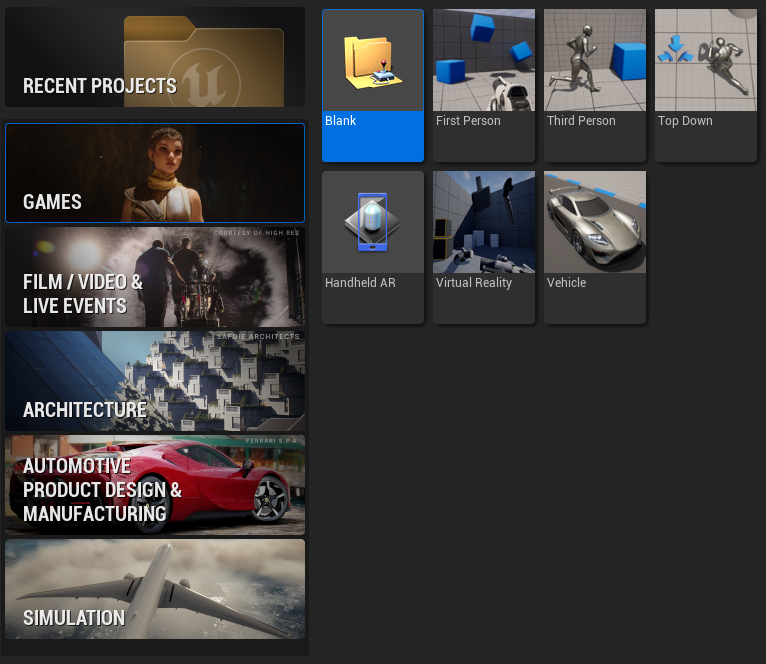
\includegraphics [width=12cm]
{continut/capitol3/figuri/UE_Templates.png} 
\caption{Proiecte de tip "template"} 
\label{fig:VR_Templates} 
\end{figure}

Un proiect în Unreal Engine 5 începe prin alegerea unui șablon de bază, organizat în funcție de scopul aplicației. Motorul oferă o serie de categorii predefinite care acoperă o gamă largă de domenii, de la dezvoltarea de jocuri până la aplicații industriale și vizualizari arhitecturale. 

\begin{itemize}
\item \textbf{Games} - este utilizată în principal pentru dezvoltarea de jocuri video și experiențe interactive. Aceasta a fost și opțiunea selectată pentru proiectul de față - VR Museum - datorită flexibilității și compatibilității cu template-ul „Virtual Reality”. Majoritatea dezvoltatorilor din industria de gaming aleg această categorie pentru prototipuri și produse finale. Jocuri comerciale de renume precum Fortnite, Valorant sau Poppy Playtime sunt exemple concrete ale utilizării Unreal Engine în producția de jocuri ”AAA” sau ”Indie”.
\item \textbf{Film / Video \& Live Events} - crearea de efecte vizuale și medii digitale pentru producții cinematografice sau evenimente live poate fi extrem de costisitoare, mai ales când se folosesc decoruri reale. Unreal Engine oferă instrumente avansate pentru previzualizare, in-camera VFX și integrare cu LED volume, reducând astfel costurile de producție și timpul de execuție. Un exemplu notabil este utilizarea Unreal Engine în realizarea unor secvențe din serialul ”The Mandalorian” (Star Wars), unde fundalurile generate în timp real au înlocuit decorurile tradiționale.
\item \textbf{Architecture} - categoria dedicată arhitecturii permite crearea de vizualizări realiste pentru proiecte de construcții și design interior. Aceasta oferă integrare nativă cu instrumente CAD și BIM (precum Revit, ArchiCAD), prin intermediul Datasmith. Se pot crea schițe interactive, simulări de iluminare naturală și tururi virtuale, facilitând colaborarea dintre arhitecți, designeri și clienți. Această abordare reduce riscul de erori și crește eficiența în procesul decizional.
\item \textbf{Automotive Product Design \& Manufacturing} - este conceput special pentru industria auto, acoperind atât partea de vizualizare a designului vehiculului, cât și prototiparea interfețelor grafice utilizate în habitaclu (HMI - Human-Machine Interface). De exemplu, Mercedes-Benz utilizează Unreal Engine în dezvoltarea interfeței digitale MBUX Hyperscreen, un sistem avansat care rulează pe un ecran panoramic. De asemenea, General Motors integrează Unreal în platforma Ultium, utilizată în vehicule electrice precum Cadillac și Hummer EV, pentru a genera în timp real animații și interacțiuni în bordul mașinii.
\item \textbf{Simulation} - destinată dezvoltării de simulatoare pentru aplicații educaționale, industriale sau de formare profesională. Unreal Engine permite integrarea fizicii avansate, a senzorilor virtuali și a scenariilor dinamice. Aceasta este utilizată, de exemplu, pentru simulatoare de zbor, simulatoare auto (pentru camioane, trenuri etc.) sau pentru programe de instruire în medii controlate, precum aplicațiile medicale sau militare. Realismul oferit de motorul grafic contribuie la crearea unor experiențe imersive și credibile, utile în formarea personalului specializat.

\end{itemize}

Categoria Games din Unreal Engine 5 este destinată proiectelor interactive, în special jocurilor video. Ea oferă mai multe șabloane (templates) predefinite care acoperă diverse tipuri de gameplay și stiluri de joc. Alegerea unui template potrivit poate accelera procesul de prototipare și dezvoltare, oferind o bază funcțională adaptată nevoilor proiectului. Dintre acestea, cele mai utilizate sunt:

\begin{itemize}
\item \textbf{Blank} - oferă un proiect complet gol, fără personaje, logică de joc sau componente suplimentare. Este potrivit pentru dezvoltatori care doresc să construiască o experiență complet personalizată, de la zero, fără a fi constrânși de o structură predefinită.
\item \textbf{First Person} - este utilizat pentru jocuri de tip shooter sau explorare. Include un personaj preconfigurat, cu posibilitatea de a interacționa cu obiecte, a sări și a trage cu un proiectil. Un exemplu de joc popular dezvoltat în Unreal Engine care folosește perspectiva first person este Poppy Playtime.
\item \textbf{Third Person} - include un personaj văzut din spate și o cameră cinematică de urmărire. Este frecvent utilizat în jocuri narative sau de aventură. Un exemplu relevant este Tomb Raider (Shadow of the Tomb Raider), dezvoltat parțial folosind Unreal Engine, care utilizează această perspectivă pentru a crea o experiență dinamică.
\item \textbf{Top Down} - presupune o cameră plasată deasupra personajului, ideal pentru jocuri tactice, RPG-uri sau strategie în timp real. Exemple de astfel de jocuri sunt Transistor și The Ascent, care adoptă această perspectivă pentru a oferi o viziune strategică asupra mediului.
\item \textbf{Handheld AR} - orientat spre aplicații de realitate augmentată (AR) pe dispozitive mobile. Permite recunoașterea planurilor reale și plasarea obiectelor 3D în spațiul fizic. Exemple de aplicații similare includ Pokémon GO, Minecraft Earth, sau funcționalitatea View in 3D/AR oferită de Google Search, unde utilizatorii pot vizualiza animale, obiecte sau produse în propriul mediu, prin camera telefonului.
\item \textbf{Vehicle} - conține o logică de conducere a unui vehicul cu roți și suspensii fizice. Este folosit în dezvoltarea jocurilor de tip racing sau simulatoare de condus. Printre exemplele celebre se numără GRIP: Combat Racing sau Next Car Game: Wreckfest, care folosesc componente fizice avansate pentru a simula comportamentul realist al vehiculelor.
\item \textbf{Virtual Reality (VR)} - acest template este special conceput pentru dezvoltarea de aplicații în realitate virtuală, compatibil cu standardul OpenXR. Include funcționalități precum teleportarea, interacțiunea cu obiecte (grab), meniuri 3D și suport pentru modul spectator. În cadrul lucrării de licență, acest template a fost ales ca punct de plecare pentru realizarea aplicației VR Museum. Detaliile tehnice și funcționale ale acestui șablon vor fi prezentate în secțiunile următoare.

\end{itemize}

\section{Structura și funcționalitățile șablonului VR Template}

Șablonul Virtual Reality Template oferit de Unreal Engine 5 este un punct de plecare extrem de util pentru dezvoltatorii care doresc să creeze experiențe imersive în realitate virtuală. Acesta vine preconfigurat cu o serie de funcționalități esențiale pentru interacțiunea naturală în medii tridimensionale, permițând un timp de dezvoltare redus și o adaptabilitate ridicată pentru diverse tipuri de proiecte VR.

\begin{figure}[h!]
    \centering
    \begin{subfigure}{0.49\textwidth}
        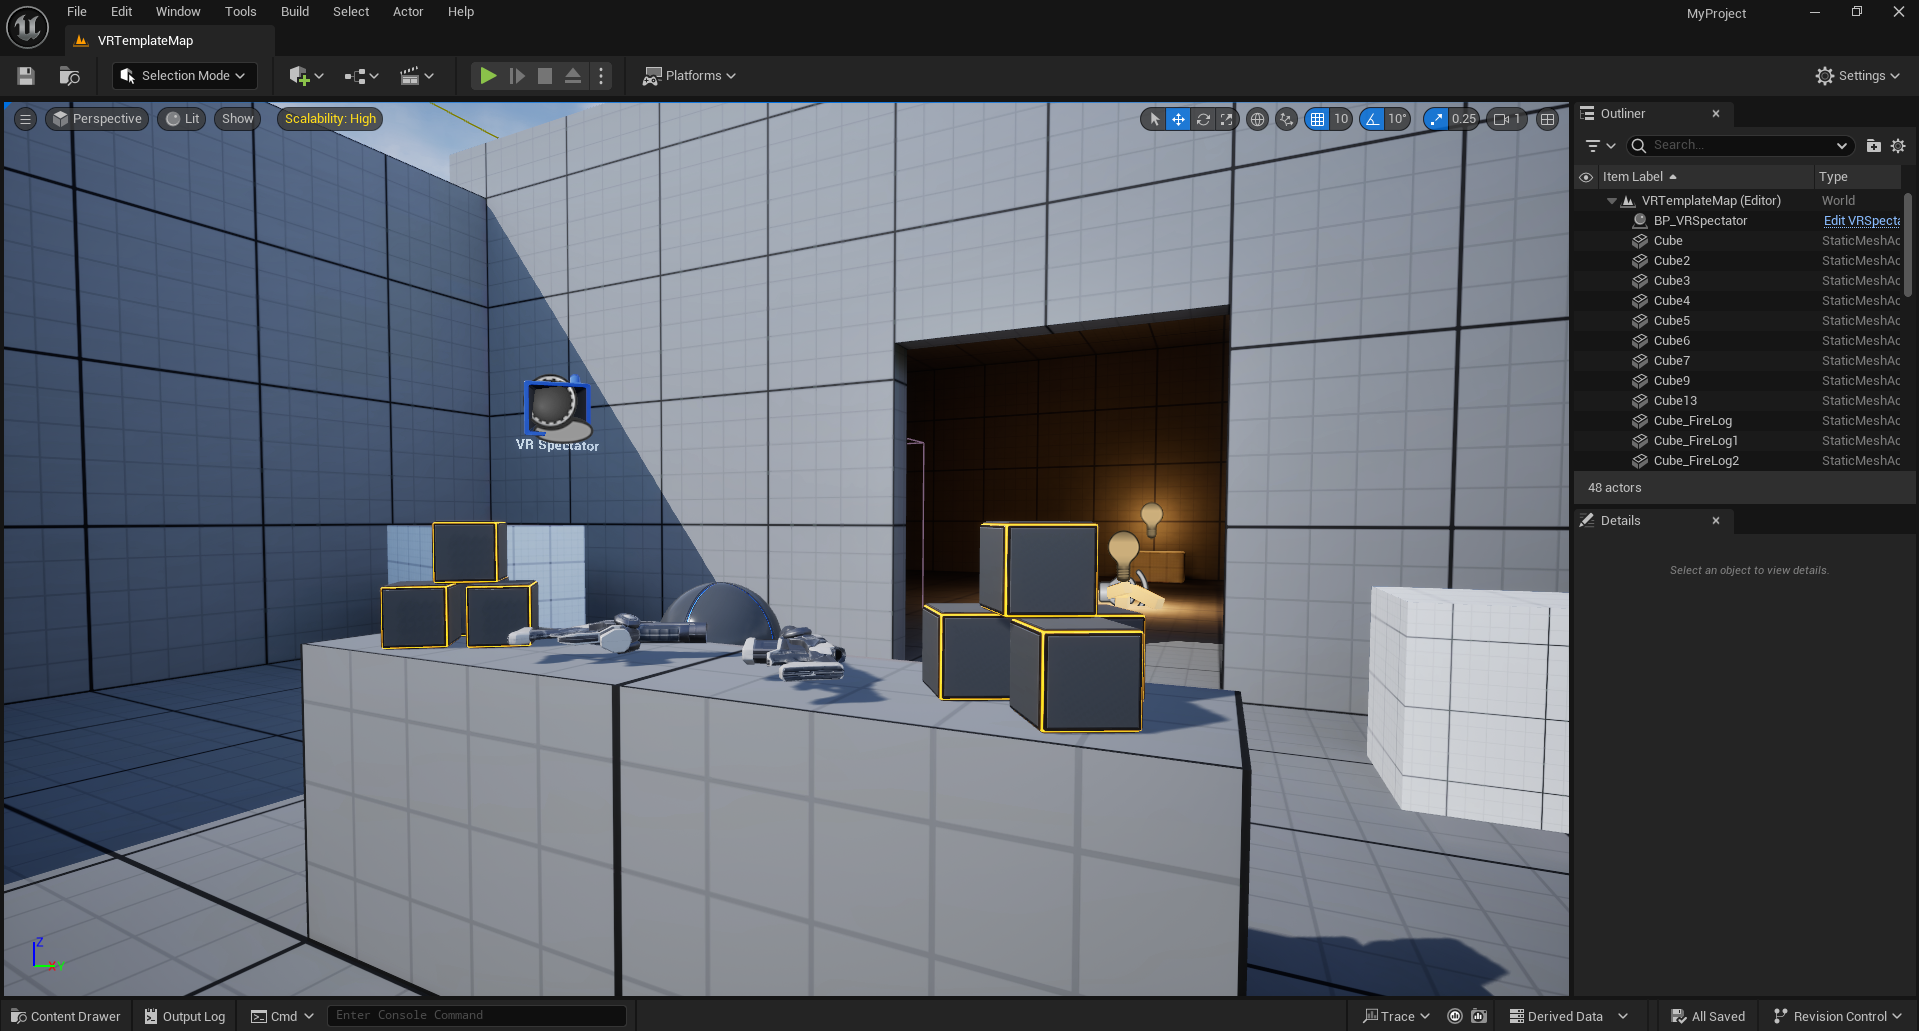
\includegraphics[width=\linewidth, height=6cm]{continut/capitol3/figuri/VR_front.png}
        \label{fig:VR Template}
    \end{subfigure}
    \hfill
    \begin{subfigure}{0.49\textwidth}
        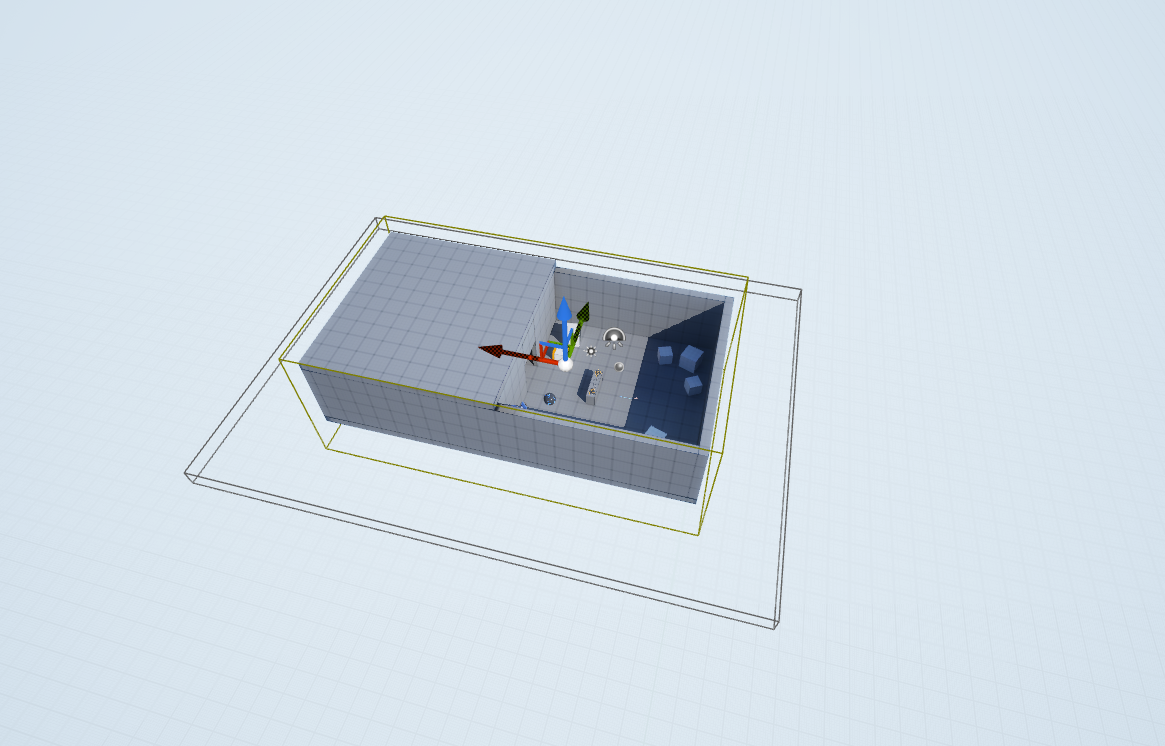
\includegraphics[width=\linewidth, height=6cm]{continut/capitol3/figuri/VR_up.png}
        \label{fig:VR Template}
    \end{subfigure}

    \caption{VR Template}
\end{figure}

Proiectul generat pe baza acestui șablon include o scenă simplă, structurată în două zone: una interioară, asemănătoare unei camere, și una exterioară, expusă la cer. În interiorul scenei se regăsesc mai multe obiecte 3D, unele dintre acestea fiind interactive - pot fi apucate (grab) și manipulate cu ajutorul controlerelor VR. Interacțiunea se realizează natural, prin folosirea butonului de prindere de pe manetă, iar obiectele reacționează în funcție de tipul definit în sistemul de prindere (Snap sau Free Grab).

În zona interioară este prezent un element ambiental format dintr-un foc de tabără. Acesta este compus din câteva cărămizi care simulează reflexii luminoase dinamice și un efect sonor realist ce imită sunetul lemnelor care ard. Aceste elemente contribuie la crearea unei atmosfere imersive și ajută la testarea performanței aplicației în condiții diverse de lumină și sunet.

Locomoția în această experiență se realizează printr-o metodă standard de deplasare în VR, numită teleportare. Utilizatorul poate activa acest sistem prin joystick-ul de pe maneta stângă. În momentul acționării, din mâna stângă este proiectată o linie vizuală ce indică direcția și destinația dorită. După selectarea poziției, teleportarea are loc în momentul eliberării joystick-ului. Sistemul este configurabil, putând fi ajustate zona de destinație, raza de teleportare sau feedback-ul vizual.

Pe lângă deplasare, șablonul integrează și un sistem de rotație incrementală, acționat prin joystick-ul de pe maneta dreaptă. Acesta permite utilizatorului să rotească avatarul la stânga sau la dreapta în pași predefiniți (snap turn), contribuind la reducerea disconfortului asociat cu rotația continuă în VR. Viteza și unghiul fiecărei rotații pot fi configurate în editorul Blueprint.

Template-ul include și un sistem de meniuri interactive în realitate virtuală, activate prin apăsarea unui buton dedicat de pe controler. Acestea sunt afișate sub forma unor ferestre 3D, care pot fi poziționate în fața utilizatorului și utilizate pentru setări, navigare sau informații suplimentare.

Din punct de vedere tehnic, proiectul conține mai multe Blueprint-uri predefinite, fiecare responsabil pentru funcționalitățile principale: deplasarea prin teleport, rotația incrementală, sistemul de prindere a obiectelor și gestionarea meniurilor. Acestea sunt ușor de înțeles și de personalizat, fiind bine documentate atât în interiorul editorului, cât și prin surse externe.

Alegerea acestui template a avut un impact semnificativ în simplificarea procesului de dezvoltare. Deși toate funcționalitățile prezentate puteau fi construite manual de la zero, utilizarea unui cadru existent a permis focalizarea pe aspectele creative și educaționale ale proiectului. În plus, VR Template beneficiază de o comunitate activă și o bază solidă de documentație oficială oferită de Epic Games, ceea ce a facilitat învățarea și adaptarea rapidă în cadrul proiectului VR Museum.

\section{Cadrul virtual}

În cadrul experienței virtuale VR Museum, utilizatorul are posibilitatea de a explora un muzeu de istorie naturală într-un mediu imersiv, conceput pentru a oferi atât elemente educaționale, cât și momente de descoperire interactivă. Totuși, forma actuală a proiectului nu a fost prezentă de la început; inițial, direcția aleasă a fost una mai ambițioasă și complexă, dar dificil de realizat în condițiile tehnice disponibile.

\begin{figure}[h!]
    \centering
    \begin{subfigure}{0.49\textwidth}
        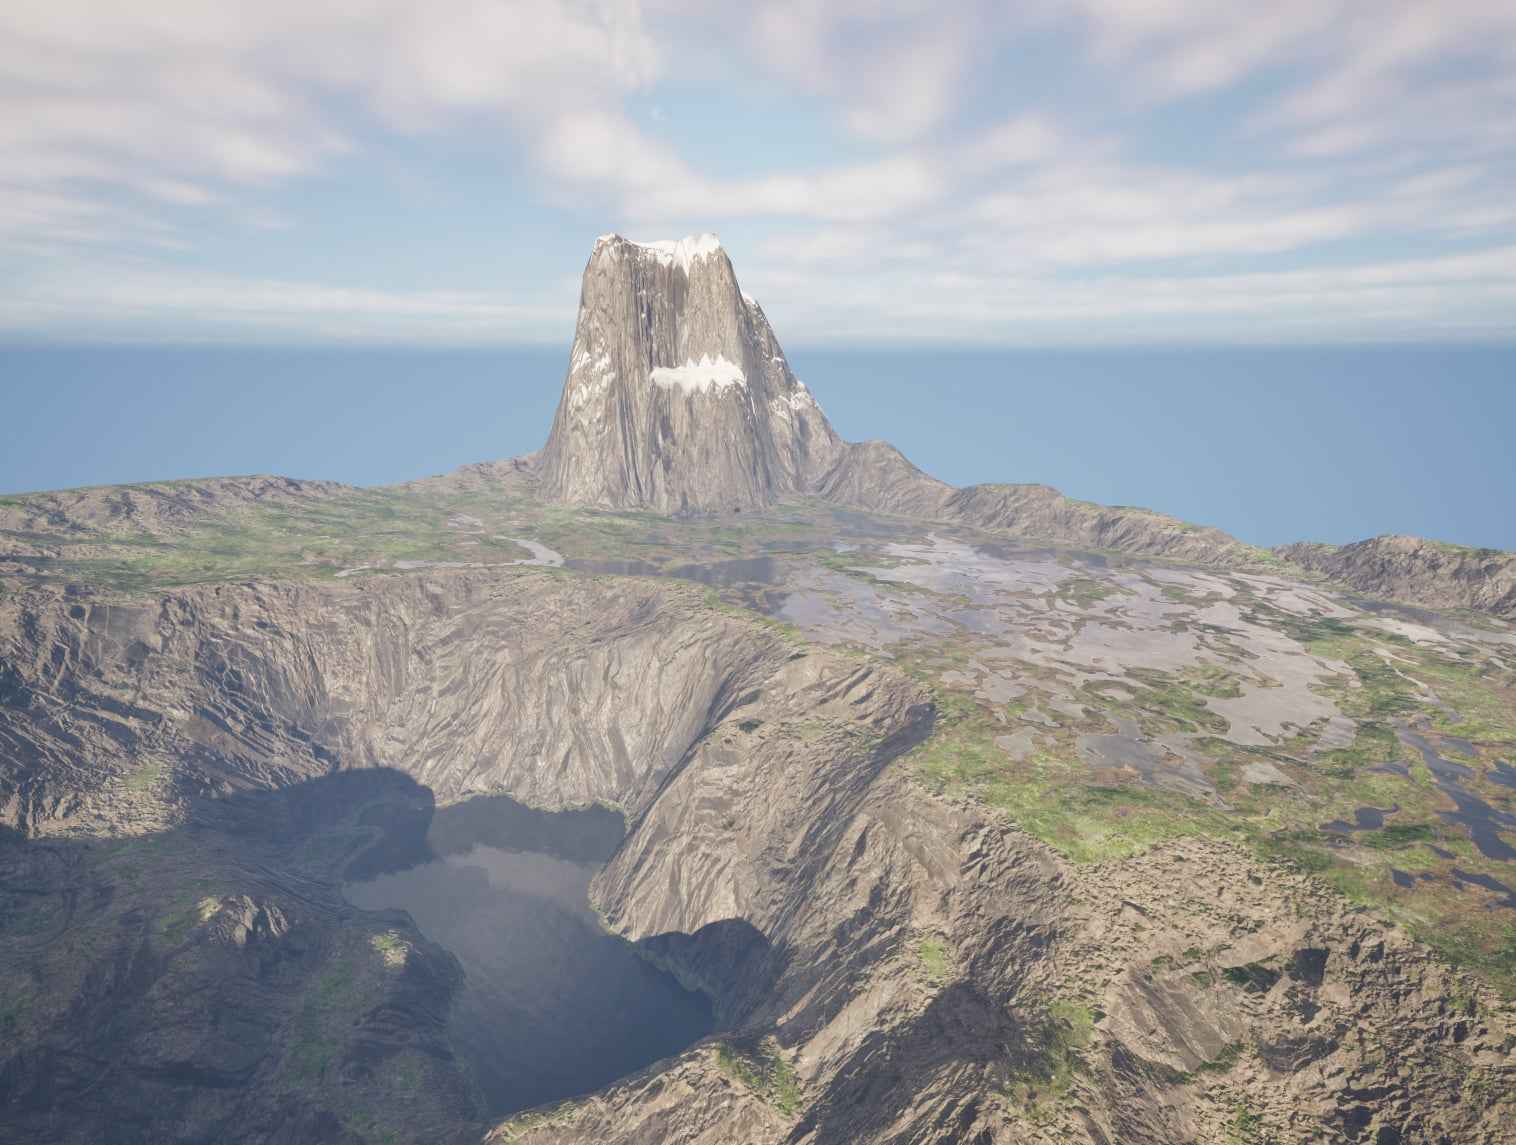
\includegraphics[width=\linewidth, height=6cm]{continut/capitol3/figuri/attempt.jpg}
        \label{fig:First VR attempt}
    \end{subfigure}
    \hfill
    \begin{subfigure}{0.49\textwidth}
        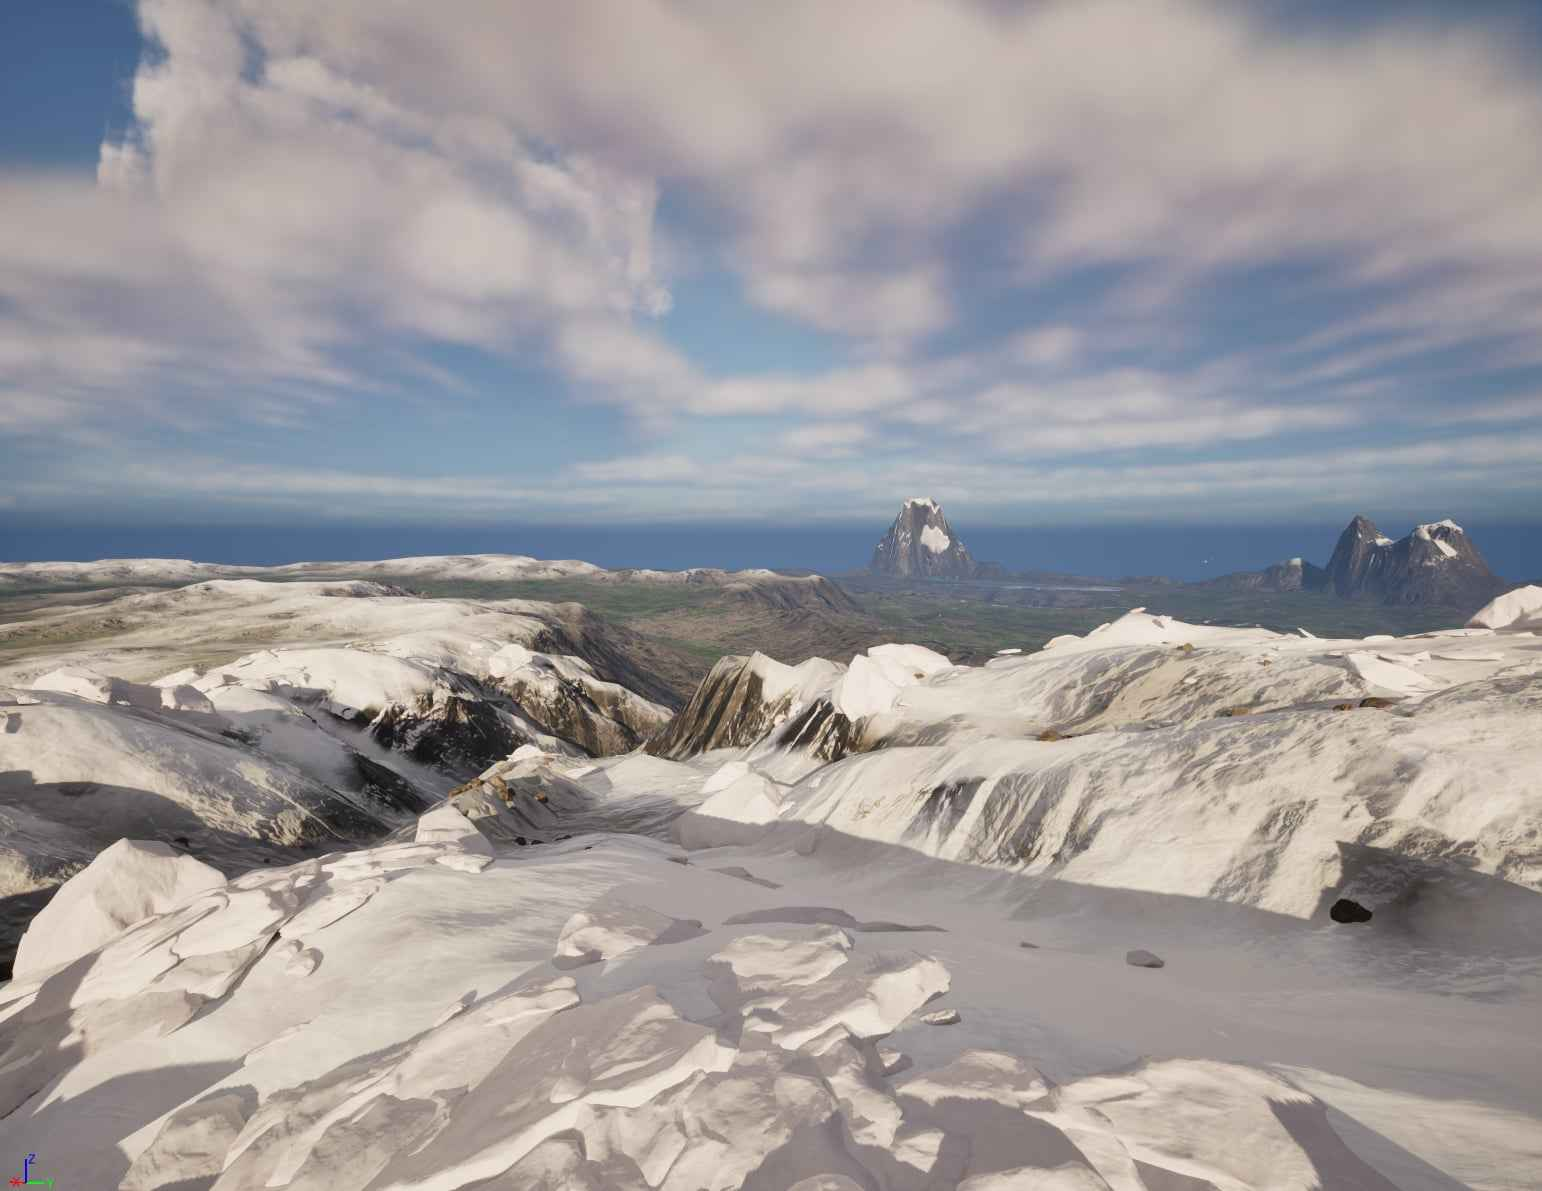
\includegraphics[width=\linewidth, height=6cm]{continut/capitol3/figuri/attempt1jpg.jpg}
        \label{fig:First VR attempt}
    \end{subfigure}

    \caption{Proiecutl initial}
\end{figure}

Versiunea inițială a proiectului includea un spațiu extins, compus dintr-o încăpere de pornire de dimensiuni reduse, care acționa ca un punct de introducere, urmat de o zonă largă, asemănătoare unei poieni deschise, unde utilizatorul putea explora mai multe expoziții dedicate dinozaurilor. Peisajul era vast și detaliat, oferind impresia unui mediu natural neîngrădit, departe de civilizația cotidiană. Deși zonele periferice ale scenei nu erau accesibile direct, designul acestora contribuia la senzația de profunzime și izolare - un spațiu fictiv, dar credibil, menit să stimuleze curiozitatea și să creeze atmosfera unei călătorii în timp.

Fiecare expoziție era dedicată unei specii de dinozaur, prezentând o combinație între modelul tridimensional al animalului și informații descriptive. Panourile interactive amplasate în jurul exponatului ofereau detalii despre perioada în care trăia specia respectivă, obiceiuri alimentare, habitat și descoperiri științifice relevante. Printre aceste panouri se regăsea și un buton intitulat „Preview”, a cărui funcție era să teleporteze utilizatorul într-un mediu special recreat pentru acea epocă istorică. Aceste scene tematice simulau condițiile de mediu - vegetație preistorică, climă, iluminare specifică și chiar sunete ambientale precum ciripitul reptilelor primitive sau foșnetul frunzelor mari - totul gândit pentru a oferi o experiență completă și educativă.

În anumite cazuri, scena „preview” includea și o formă limitată de interacțiune: utilizatorul putea observa dinozaurul în mișcare, putea urmări o simulare de comportament specific (de exemplu, hrănire sau apărare), iar unele elemente ale mediului răspundeau la acțiunile acestuia (de exemplu, vegetația se mișca la apropiere). Această abordare avea scopul de a oferi nu doar o experiență pasivă de vizionare, ci una activă, bazată pe explorare și imersiune contextuală.

Astfel, s-a optat pentru o variantă mai realistă și fezabilă: un muzeu structurat în principal ca un spațiu interior, dar care include și o componentă exterioară. Această alegere a permis organizarea expozițiilor într-un mod mai coerent și ușor de gestionat, fără a compromite scopul educativ sau caracterul interactiv al experienței. De asemenea, am putut investi mai mult timp în perfecționarea accesibilității - prin optimizarea controalelor, a interfeței și a performanței aplicației - și în atragerea unui public mai larg, inclusiv utilizatori care nu sunt familiarizați cu tehnologia VR.

Prin această tranziție de la o idee conceptuală ambițioasă către o execuție practică și focalizată, proiectul VR Museum a reușit să păstreze esența scopului său - educarea prin explorare imersivă - fără a compromite stabilitatea, claritatea și calitatea experienței finale.

Pentru implementarea proiectul, s-a construit cladirea in care vor fi adaugate restul de obiecte, expozitii, etc.

\section{Alcatuirea muzeului și a spațiului înconjurător}

\begin{figure} [htp] 
\centering 
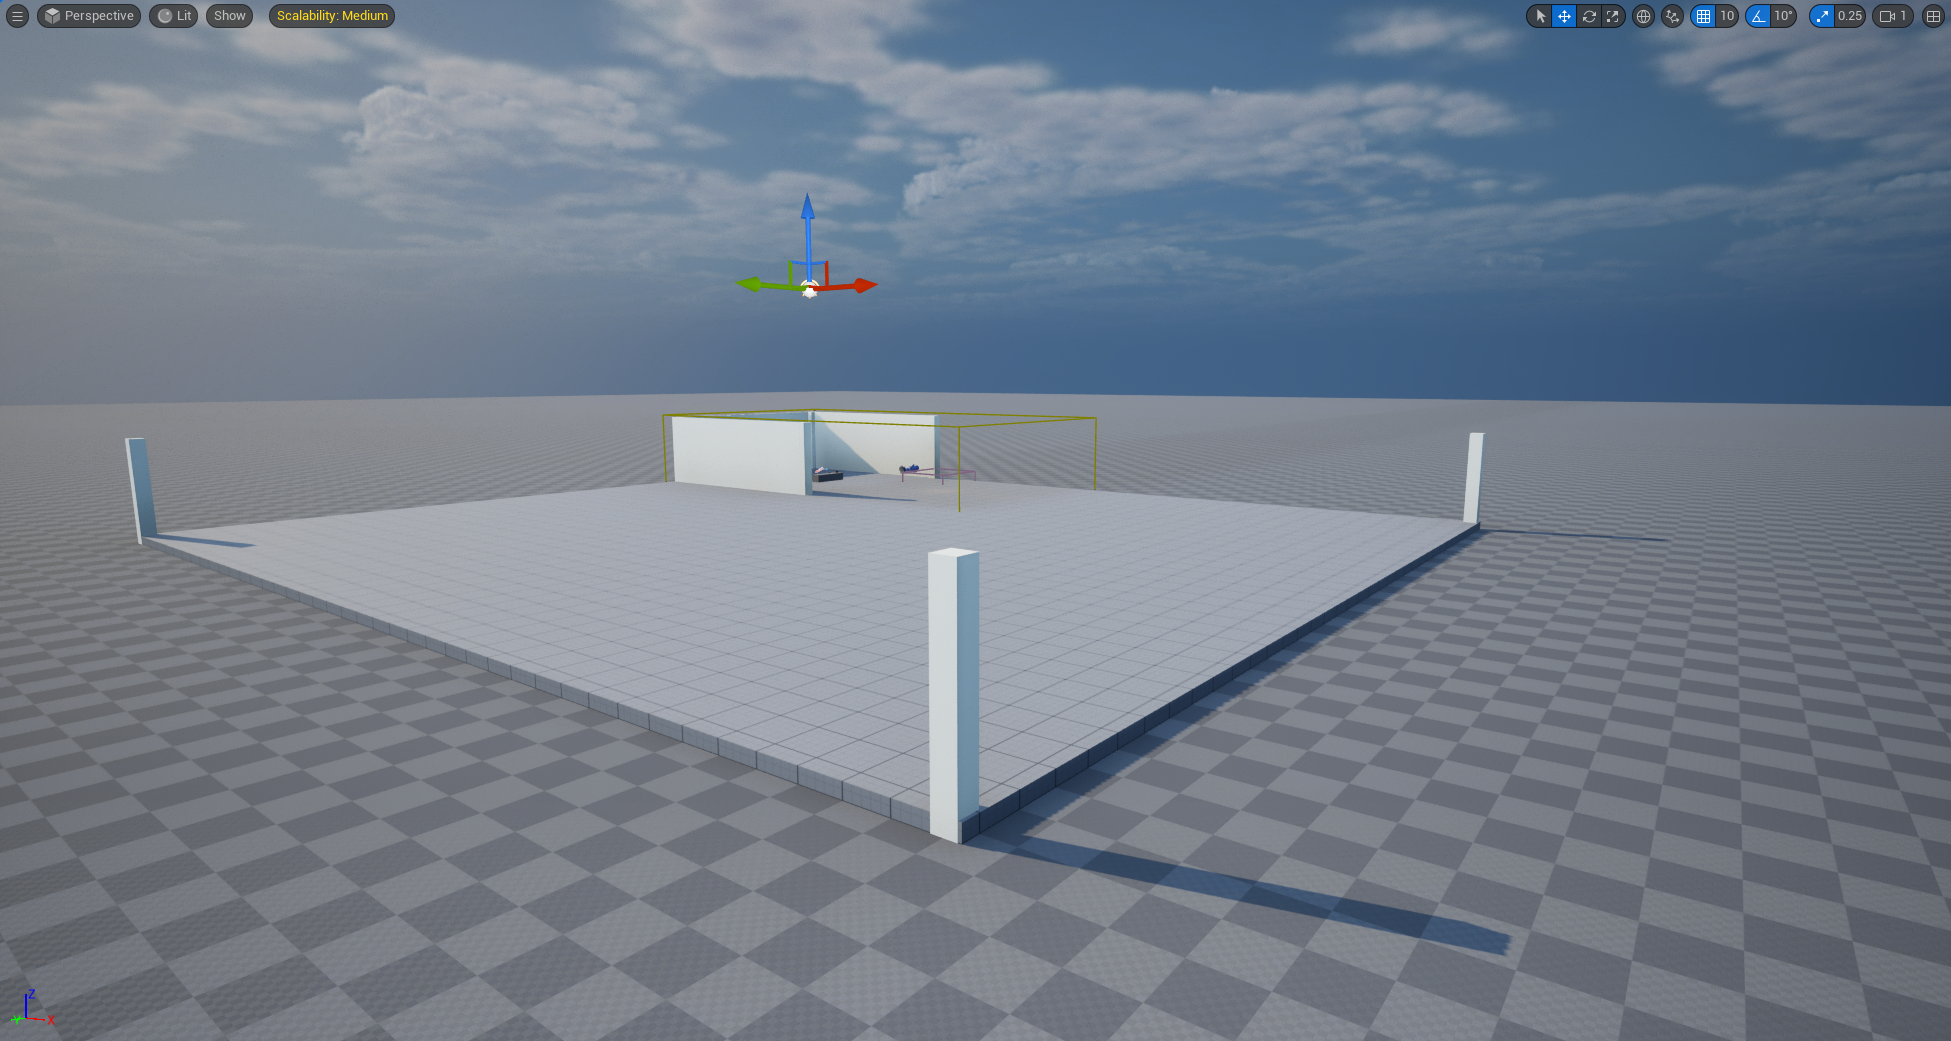
\includegraphics [width=12cm]
{continut/capitol3/figuri/beginning.png} 
\caption{Alcătuirea muzeului} 
\label{fig:Museum} 
\end{figure}

Arhitectura muzeului a fost construită utilizând obiectele disponibile în pachetul StarterContent, oferit gratuit odată cu șablonul Unreal Engine. Aceste elemente de bază au constituit punctul de plecare pentru amenajarea spațiului interior, fiind alese pentru simplitatea integrării și compatibilitatea directă cu structura proiectului.
\begin{figure}[h!]
    \centering
    \begin{subfigure}{0.49\textwidth}
        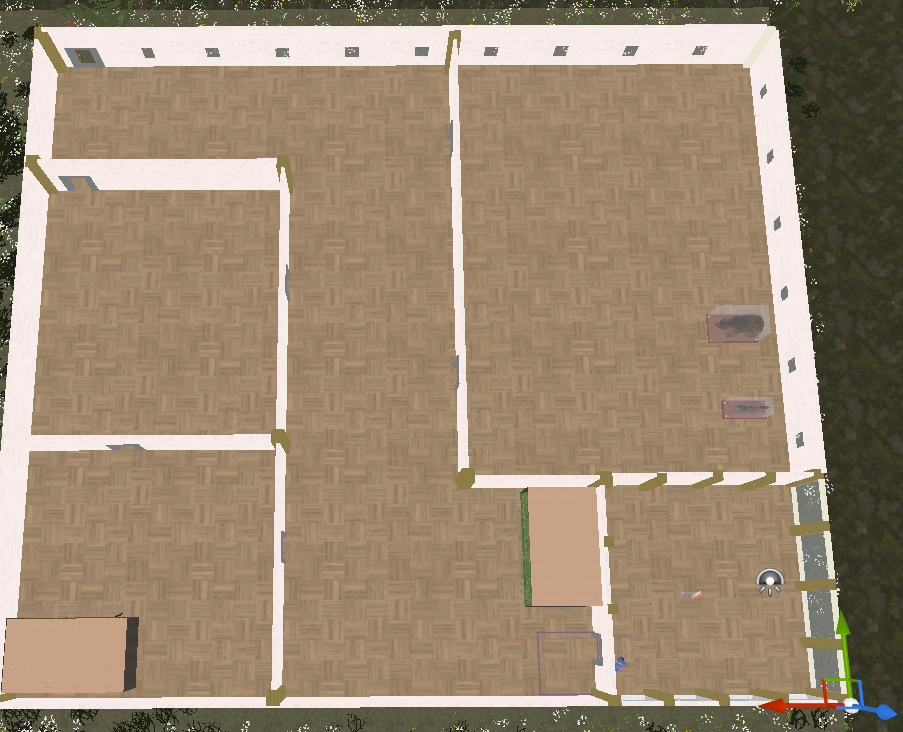
\includegraphics[width=\linewidth, height=6cm]{continut/capitol3/figuri/scheme.png}
        \label{fig:Museum}
    \end{subfigure}
    \hfill
    \begin{subfigure}{0.49\textwidth}
        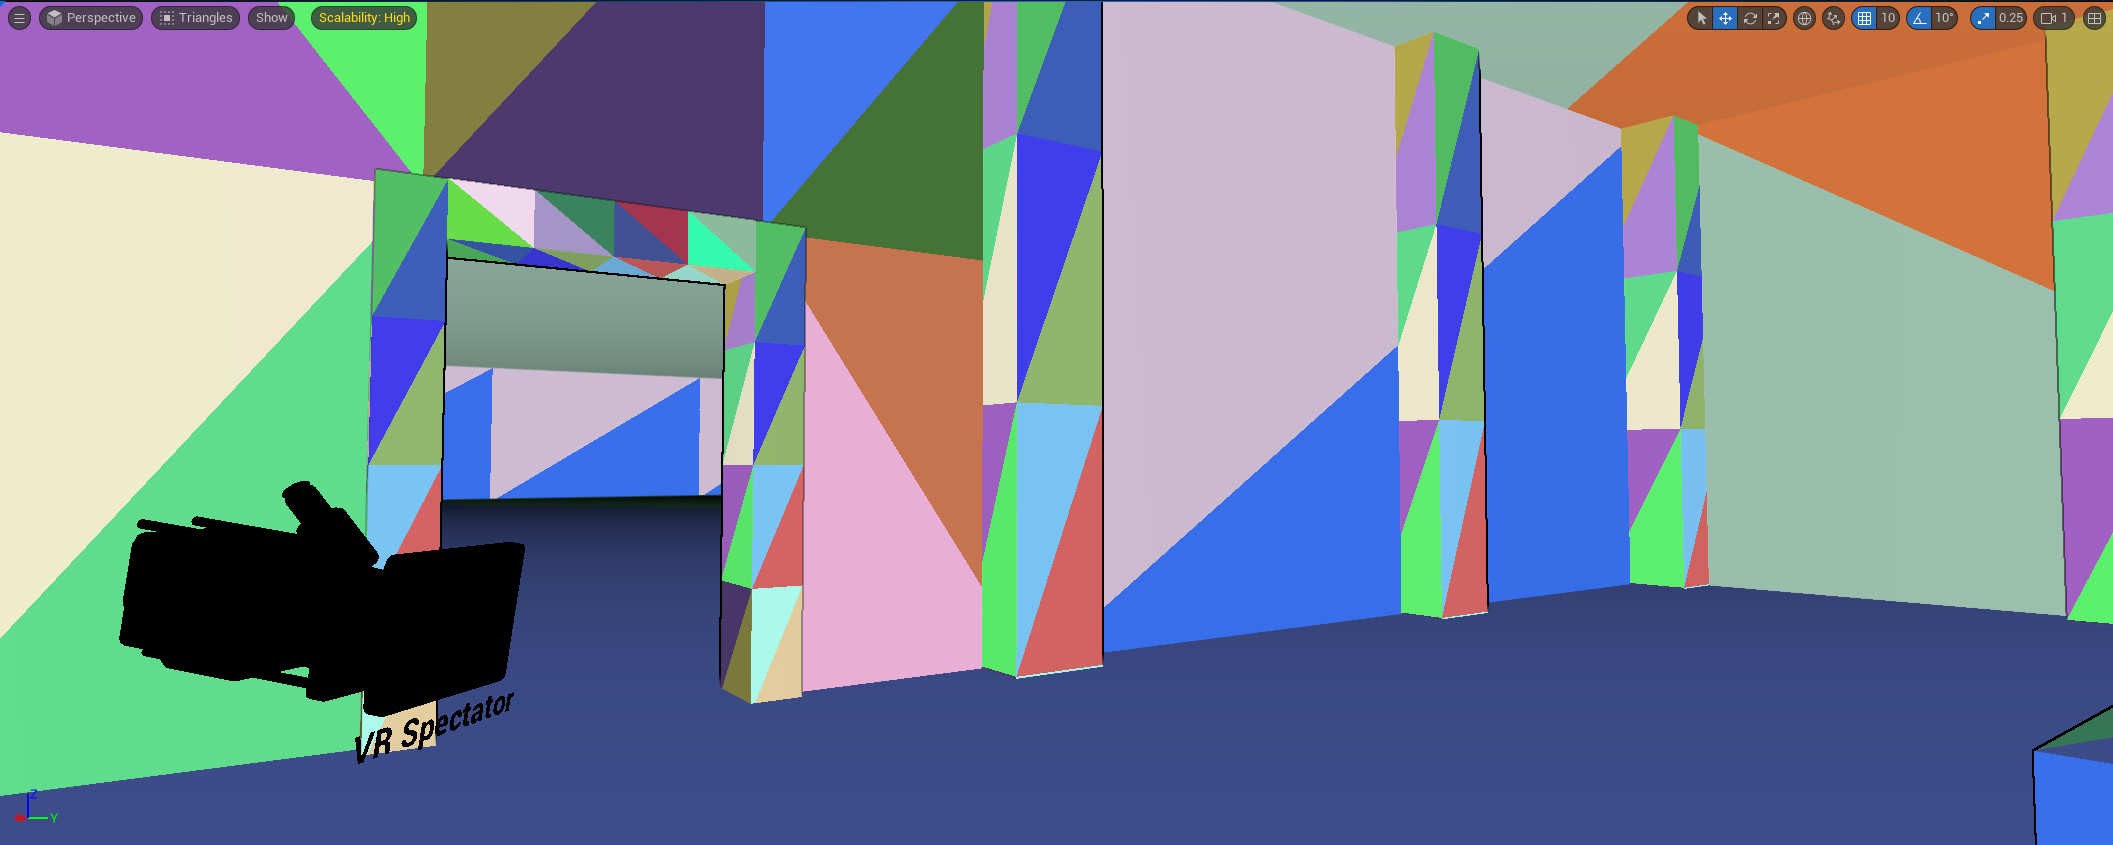
\includegraphics[width=\linewidth, height=6cm]{continut/capitol3/figuri/Screenshot 2025-03-03 135626.png}
        \label{fig:Museum}
    \end{subfigure}
    \caption{Alcătuirea mzeului - camera si utilizarea tehnologii Nanite pentru modelarea obiectelor}
\end{figure}

\begin{figure}[h!]
    \centering
    \begin{subfigure}{0.49\textwidth}
        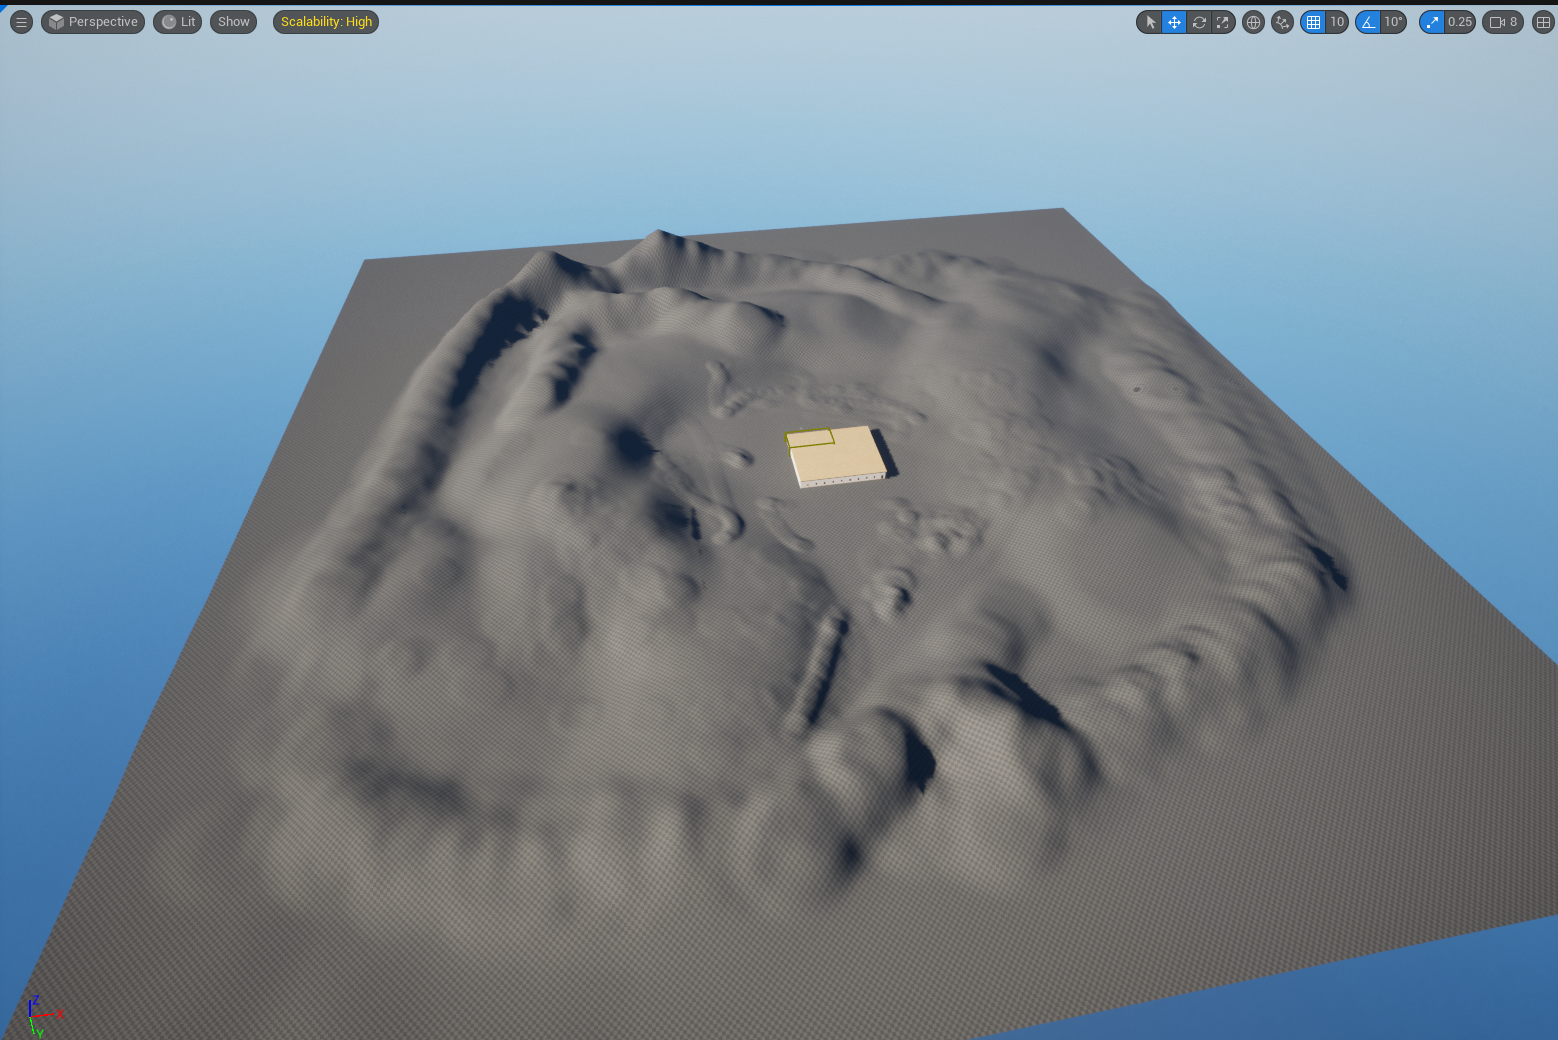
\includegraphics[width=\linewidth, height=6cm]{continut/capitol3/figuri/3_terrain_mapping.png}
        \label{fig:Terrain mapping}
    \end{subfigure}
    \hfill
    \begin{subfigure}{0.49\textwidth}
        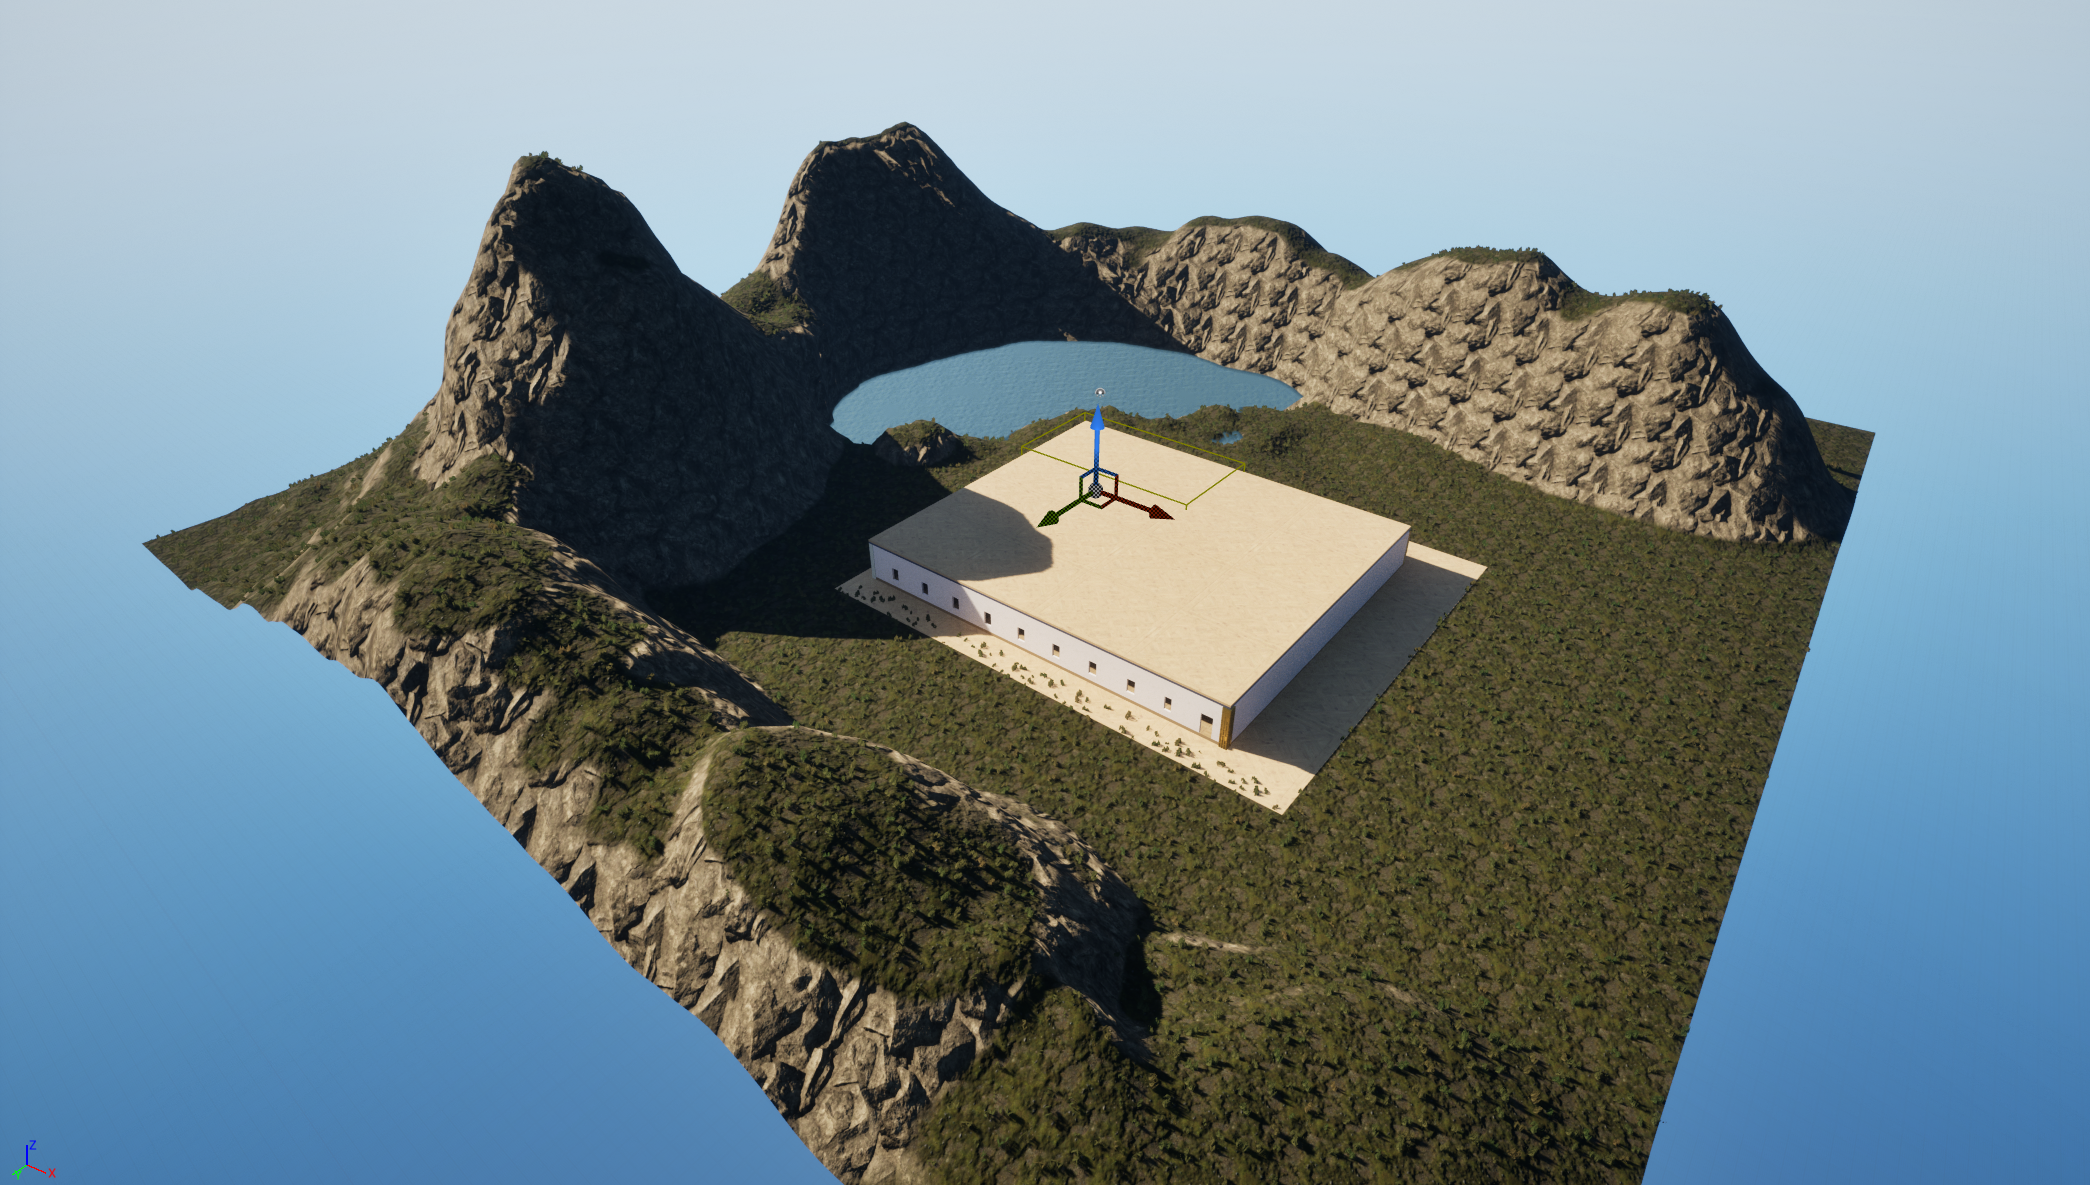
\includegraphics[width=\linewidth, height=6cm]{continut/capitol3/figuri/4_terrain_texture.png}
        \label{fig:Terrain mapping}
    \end{subfigure}
    \begin{subfigure}{0.49\textwidth}
        \includegraphics[width=\linewidth, height=6cm]{continut/capitol3/figuri/5_terrain_props.png}
        \label{fig:Terrain mapping}
    \end{subfigure}
    \begin{subfigure}{0.49\textwidth}
        \includegraphics[width=\linewidth, height=6cm]{continut/capitol3/figuri/6_state.png}
        \label{fig:Terrain mapping}
    \end{subfigure}

    \caption{Alcătuirea terenului}
\end{figure}
Procesul de organizare a spațiului a fost unul provocator. Deși ideile de design erau numeroase, găsirea unei soluții coerente și echilibrate din punct de vedere vizual a necesitat mai multe iterații. Inițial, muzeul a fost conceput ca un spațiu mare, deschis, fără compartimentări clare, cu scopul de a oferi flexibilitate în faza de construcție. Ulterior, acest spațiu a fost adaptat și segmentat în zone distincte, în funcție de tematica expozițiilor și de traseul pe care utilizatorul îl poate urma.

După stabilirea structurii interioare, atenția a fost direcționată către mediul exterior - peisajul virtual. Crearea acestuia a reprezentat o etapă interesantă și esențială pentru coerența vizuală a proiectului. Terenul a fost modelat manual prin instrumentele de Landscape Sculpting, adăugând munți, zone depresionare, potențiale cursuri de apă și mici denivelări care să simuleze un relief realist. Scopul a fost acela de a reda un cadru cât mai apropiat de natură, cu variații subtile de altitudine și volum care să elimine senzația de artificial sau plat. Jocul de lumină pe aceste suprafețe neregulate, împreună cu materialele de sol aplicate, contribuie la crearea unei atmosfere care, pe alocuri, poate părea apropiată de realitate.

Pentru a limita zona de explorare și a păstra imersiunea, au fost adăugate margini invizibile la extremitățile hărții. Aceste bariere împiedică utilizatorul să părăsească zona activă sau să observe capătul scenei, evitând astfel senzația că spațiul virtual este „tăiat” brusc ori incomplet.

Decorarea spațiului muzeal, precum și a zonei exterioare, a implicat integrarea unei game variate de materiale și obiecte decorative. Acestea au fost atent alese pentru a crea o experiență vizuală plăcută, diversificată și convingătoare din punct de vedere estetic.

\section{Materialele in Unreal Engine}

Pentru a adăuga detalii vizuale obiectelor din cadrul experienței VR, este necesară aplicarea unor materiale. În Unreal Engine, un material reprezintă un set complex de proprietăți vizuale care determină modul în care un obiect va reflecta lumina, ce culoare va avea, cât de rugos sau lucios va părea și ce detalii de suprafață va reda.

\begin{figure}[h!]
    \centering
    \begin{subfigure}{0.49\textwidth}
        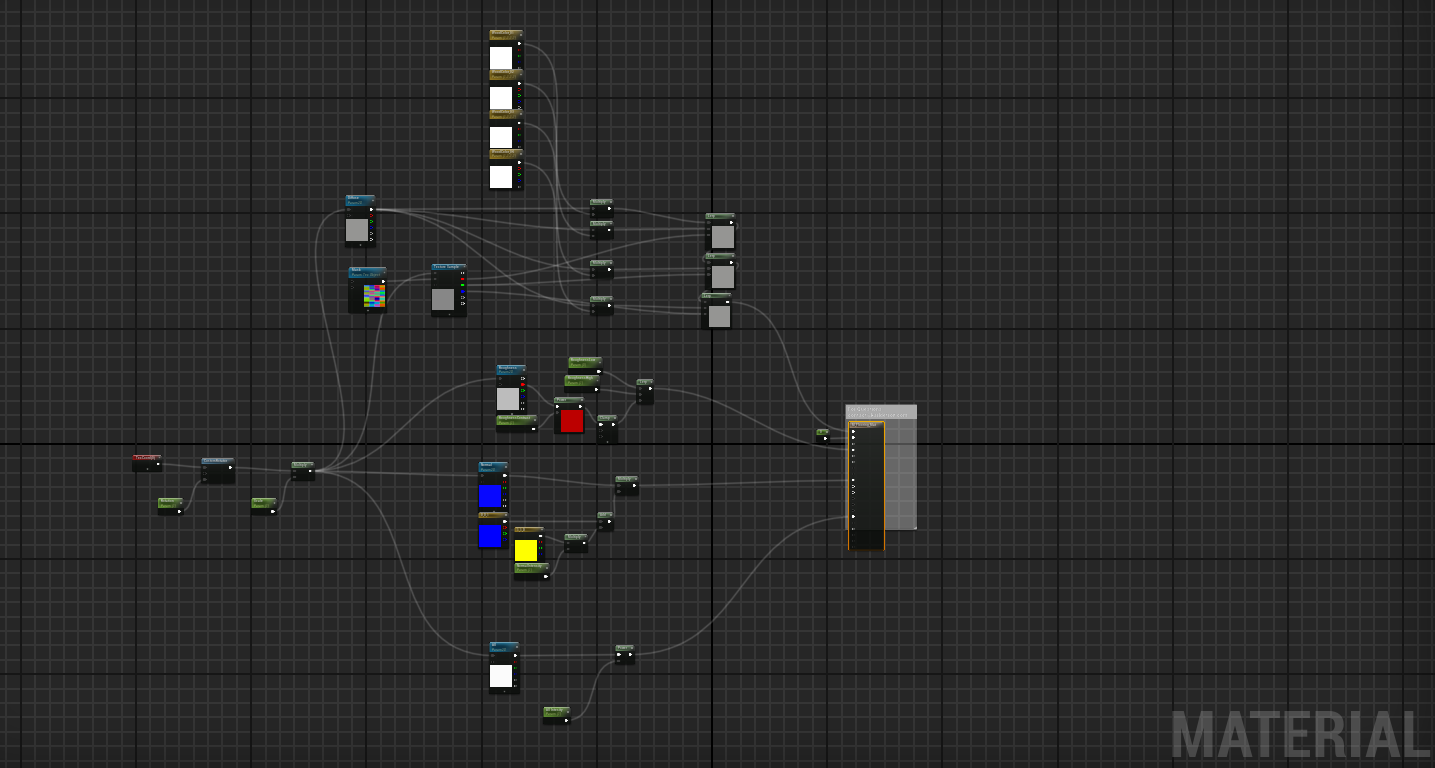
\includegraphics[width=\linewidth, height=6cm]{continut/capitol3/figuri/material.png}
        \label{fig:Terrain mapping}
    \end{subfigure}
    \hfill
    \begin{subfigure}{0.49\textwidth}
        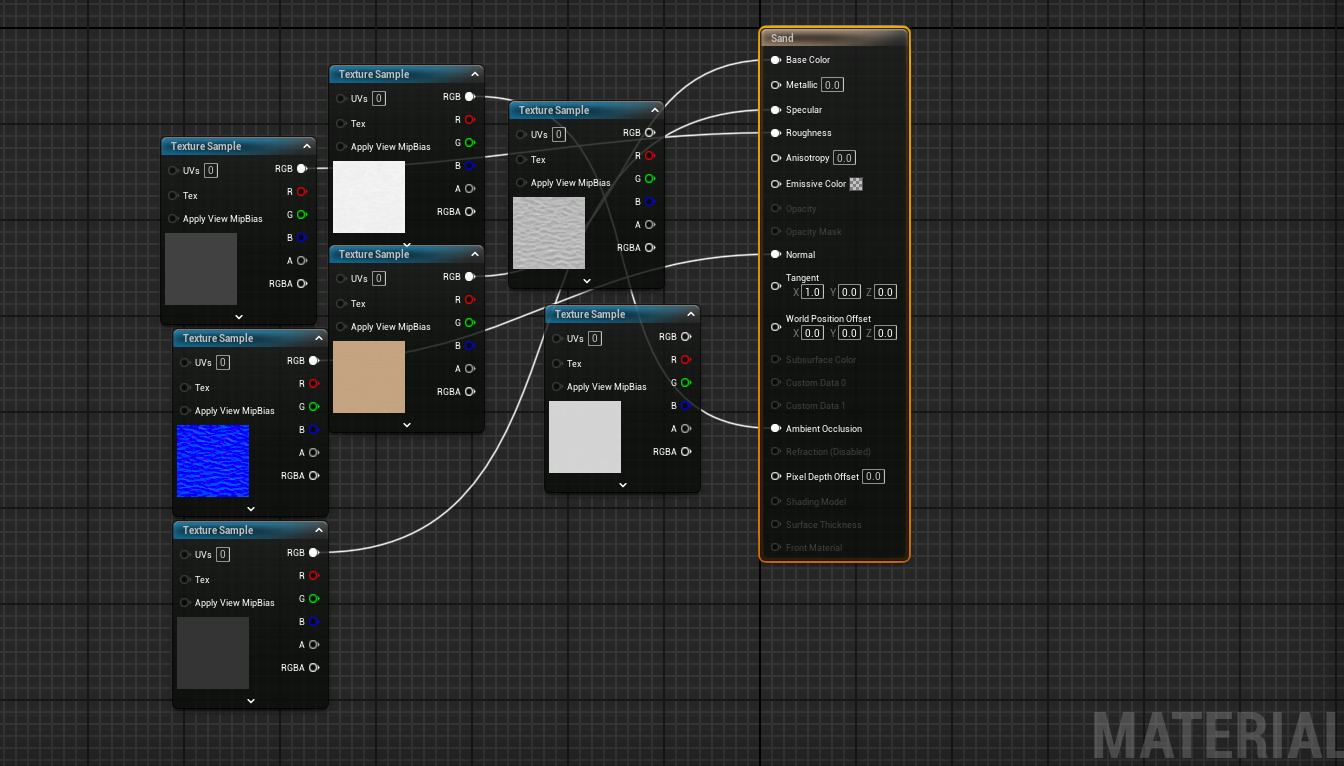
\includegraphics[width=\linewidth, height=6cm]{continut/capitol3/figuri/ez_mat.png}
        \label{fig:Terrain mapping}
    \end{subfigure}
    \caption{Un material din VR Museum}
\end{figure}

Materialele nu sunt doar culori simple aplicate pe obiecte, ci sunt compuse din mai multe texturi, fiecare având un rol specific. Aceste texturi sunt combinate într-un grafic de tip Material Editor, care permite conectarea și controlul parametrilor pentru a genera un rezultat final realist sau stilizat, în funcție de nevoile proiectului. În cele ce urmează sunt prezentate cele mai utilizate tipuri de texturi în crearea unui material de bază:

\begin{itemize}
\item \textbf{Base Color (Albedo)} - definește culoarea de bază a materialului, fără umbre sau influențe de iluminare. Este, practic, componenta vizuală dominantă care determină cum „arată” suprafața în condiții de lumină neutră. Nu conține informații despre reflexii, luciu sau profunzime, ci doar cromatică pură.
\item \textbf{Normal Map} - o textură care simulează detalii fine de suprafață, cum ar fi zgârieturi, crăpături sau muchii, fără a modifica geometria reală a obiectului. Aceasta afectează modul în care lumina interacționează cu suprafața, oferind iluzia de volum și complexitate. Este extrem de utilă în optimizarea performanței, deoarece creează detalii vizuale fără a adăuga poligoane suplimentare.
\item \textbf{Metallic} - efinește cât de metalică este suprafața materialului. Valorile ridicate (apropiate de 1) indică un material care reflectă lumina în mod specific unui metal (de exemplu, fier, aluminiu), în timp ce valorile apropiate de 0 indică un material nemetalic, cum ar fi piatra, lemnul sau plasticul. De obicei, această textură este în tonuri de gri sau alb-negru.
\item \textbf{Roughness} - controlează cât de netedă sau rugoasă este suprafața. O valoare mică (spre 0) indică o suprafață foarte lucioasă, cum ar fi sticla sau metalul lustruit, în timp ce o valoare mare (spre 1) descrie o suprafață mată și difuză, cum ar fi cimentul sau hârtia. Acest parametru influențează modul în care sunt vizibile reflexiile.
\item \textbf{Ambient Occlusion (AO)} - opțională, dar foarte utilă pentru adăugarea de umbriri fine în colțuri, margini sau zone în care lumina ambientală ar fi parțial blocată. Aceasta adaugă profunzime și realism suplimentar scenei, mai ales în combinație cu iluminarea globală.
\end{itemize}

Aceste texturi pot fi fie importate din pachete externe, fie generate procedural în editor, și sunt combinate prin noduri logice în editorul de materiale din Unreal Engine. Rezultatul final este un material care poate fi aplicat oricărui obiect 3D din scenă, contribuind esențial la aspectul general al aplicației.

În cadrul proiectului VR Museum, au fost create materiale personalizate atât pentru interiorul muzeului (parchet, pereți, vitrine), cât și pentru mediul exterior (pământ, piatră, vegetație). Fiecare material a fost adaptat pentru a reda o atmosferă coerentă și naturală, urmând principiile de bază ale physically based rendering (PBR).

Pentru crearea terenului din cadrul scenei exterioare, a fost utilizat un asset specializat, numit Landscape Pro. Acesta este un material complex, multifuncțional, care combină în mod procedural mai multe tipuri de suprafețe - pământ, iarbă și rocă - într-un singur shader aplicabil pe sistemul de landscape din Unreal Engine. Avantajul major al acestui asset constă în faptul că, odată aplicat, materialul este capabil să detecteze automat înclinația și forma reliefului și să genereze în mod procedural prop-uri decorative: fire de iarbă, ramuri uscate, frunze căzute, flori, pietre și alte elemente naturale.

Această generare procedurală nu doar că accelerează procesul de construire a unei scene realiste, dar și adaugă un nivel ridicat de detaliu și varietate, greu de obținut manual. Astfel, utilizatorul are senzația că se află într-un mediu natural credibil, viu și dinamic. Fiecare zonă a terenului este compusă dintr-o combinație vizuală de textură de sol și obiecte tridimensionale ușor diferite, ceea ce previne repetitivitatea și accentuează realismul.

Totuși, această complexitate vine cu un cost de performanță semnificativ. Landscape Pro este un material pretențios din punct de vedere al resurselor hardware, în special atunci când se folosesc setările grafice la un nivel ridicat. Obiectele generate procedural - cum ar fi iarbă, frunze sau pietre - adaugă un număr mare de instanțe care trebuie randate în timp real, ceea ce poate afecta negativ fluiditatea experienței VR pe dispozitive mai modeste. Din acest motiv, asset-ul este configurat să reacționeze la setările grafice ale aplicației: atunci când acestea sunt reduse (de exemplu, pentru a obține performanță mai bună pe sisteme cu specificații mai slabe), toate prop-urile adiționale dispar automat, rămânând doar textura de bază aplicată pe teren.

Această tranziție vizuală influențează semnificativ calitatea percepută a mediului înconjurător. La setări maxime, peisajul este bogat, divers și foarte apropiat de un mediu natural real. La setări reduse, scenele rămân funcționale, dar vizibil simplificate. Cu toate acestea, decizia de a utiliza Landscape Pro a fost una justificată de necesitatea unei prezentări vizuale impresionante, în special în contextul explorării unui muzeu în realitate virtuală, unde imersiunea este un factor esențial.

\section{Realizarea asset-urilor}

Asset-urile utilizate într-un proiect Unreal Engine pot proveni din surse variate, fie că sunt special concepute pentru motorul grafic realizat de Epic Games, fie că sunt universale și adaptate ulterior. Indiferent de proveniență, toate asset-urile 3D sunt compuse dintr-o rețea de poligoane - elemente geometrice esențiale care determină forma, complexitatea și nivelul de detaliu al obiectului. Cu cât un asset are mai multe poligoane, cu atât este mai detaliat, dar și mai costisitor din punct de vedere al performanței.

În situația ideală, asset-ul este creat special pentru Unreal Engine și vine deja optimizat, incluzând o structură internă denumită skeleton (schelet). Acest schelet permite animarea obiectului, permițând mișcarea și manipularea părților componente (cum ar fi membrele unui corp sau articulațiile unui robot). În combinație cu un set de animatii - realizate frame cu frame sau generate procedural - acest sistem oferă o bază solidă pentru personaje sau obiecte dinamice care pot reacționa la acțiunile utilizatorului sau la mediul înconjurător.

\begin{figure} [htp] 
\centering 
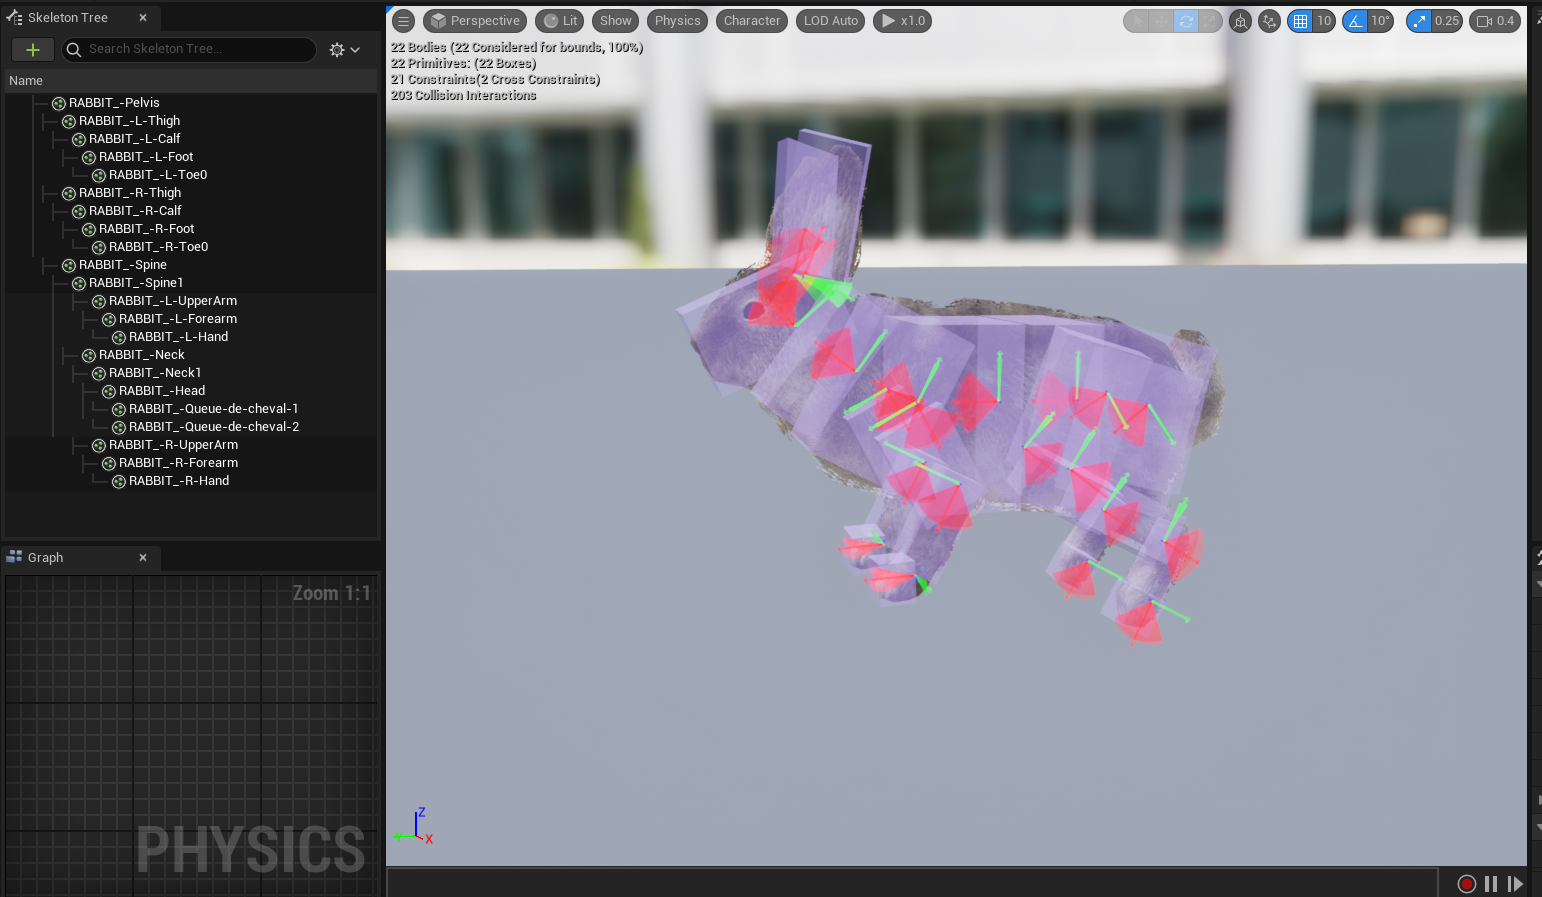
\includegraphics [width=12cm]
{continut/capitol3/figuri/rabbit.png} 
\caption{Animația unui iepure} 
\label{fig:Museum} 
\end{figure}

Pentru animarea acestor asset-uri, se folosește adesea o abordare de tip frame-by-frame, în care pozițiile oaselor și deformările de mesh sunt atent reglate pentru fiecare cadru al secvenței. Acest proces este unul laborios, care necesită precizie și atenție pentru a asigura mișcări fluide și realiste. În cazul proiectului VR Museum, însă, s-a optat pentru o soluție mai simplă: asset-urile animate au fost convertite în Static Meshes, adică obiecte statice, care nu mai pot fi animate, dar pot fi plasate direct în scenă. Această decizie a fost luată pentru a reduce complexitatea proiectului și a evita eventuale probleme de compatibilitate.

Pentru asset-urile care nu au fost concepute special pentru Unreal Engine, integrarea a presupus un proces suplimentar de convertire. Aceste resurse externe au fost descărcate din diverse surse și transformate în formatul glTF (.glb sau .gltf), unul dintre cele mai populare și versatili pentru schimbul de modele 3D. Odată convertite, ele au fost importate în editorul Unreal, însă nu fără dificultăți.

În numeroase cazuri, conversia a provocat probleme majore legate de coliziune, dimensiuni incorecte sau descompunerea asset-ului în componente multiple. Unele modele importate aveau o scară extrem de mică (ex. 0.0005), ceea ce a dus la pierderea completă a coliziunilor sau la comportamente neprevăzute în scenă. Aceste asset-uri au necesitat intervenții manuale: redimensionare, ajustare a ancorelor, eliminarea coliziunilor greșite și gruparea componentelor individuale într-un singur element logic. În unele cazuri, un singur prop era alcătuit din peste 30 de subcomponente, ceea ce a însemnat ore întregi de muncă suplimentară.

Unreal Engine suportă o varietate de formate de fișiere 3D, printre care .fbx, .glb/.gltf, .usdz sau .obj. Totuși, din toate aceste opțiuni, doar formatul glTF s-a dovedit a fi fiabil pentru fluxul de lucru folosit în acest proiect, chiar dacă au existat probleme frecvente legate de scalare și organizare internă. Formatul .fbx, deși foarte popular, a prezentat în unele cazuri erori la import, iar celelalte formate (precum .usdz) nu au oferit controlul necesar asupra parametrilor de compunere.

Integrarea asset-urilor în proiectul VR Museum a reprezentat una dintre cele mai laborioase etape ale procesului de dezvoltare. Aceasta a presupus nu doar selecția elementelor potrivite, ci și adaptarea lor la cerințele motorului grafic, corectarea manuală a erorilor și optimizarea pentru performanță, toate cu scopul de a construi un mediu coerent, atractiv vizual și funcțional în context VR.

\section{Lightning}

Pentru a asigura o atmosferă credibilă și o vizibilitate bună în cadrul experienței VR Museum, a fost implementat un sistem de iluminare mixt, care combină lumina naturală în exterior cu iluminarea artificială în interior. Alegerea acestui sistem dual are scopul de a evidenția detaliile mediului și ale expozițiilor, oferind în același timp o experiență estetică coerentă.

\begin{figure}[h!]
    \centering
    \begin{subfigure}{0.49\textwidth}
        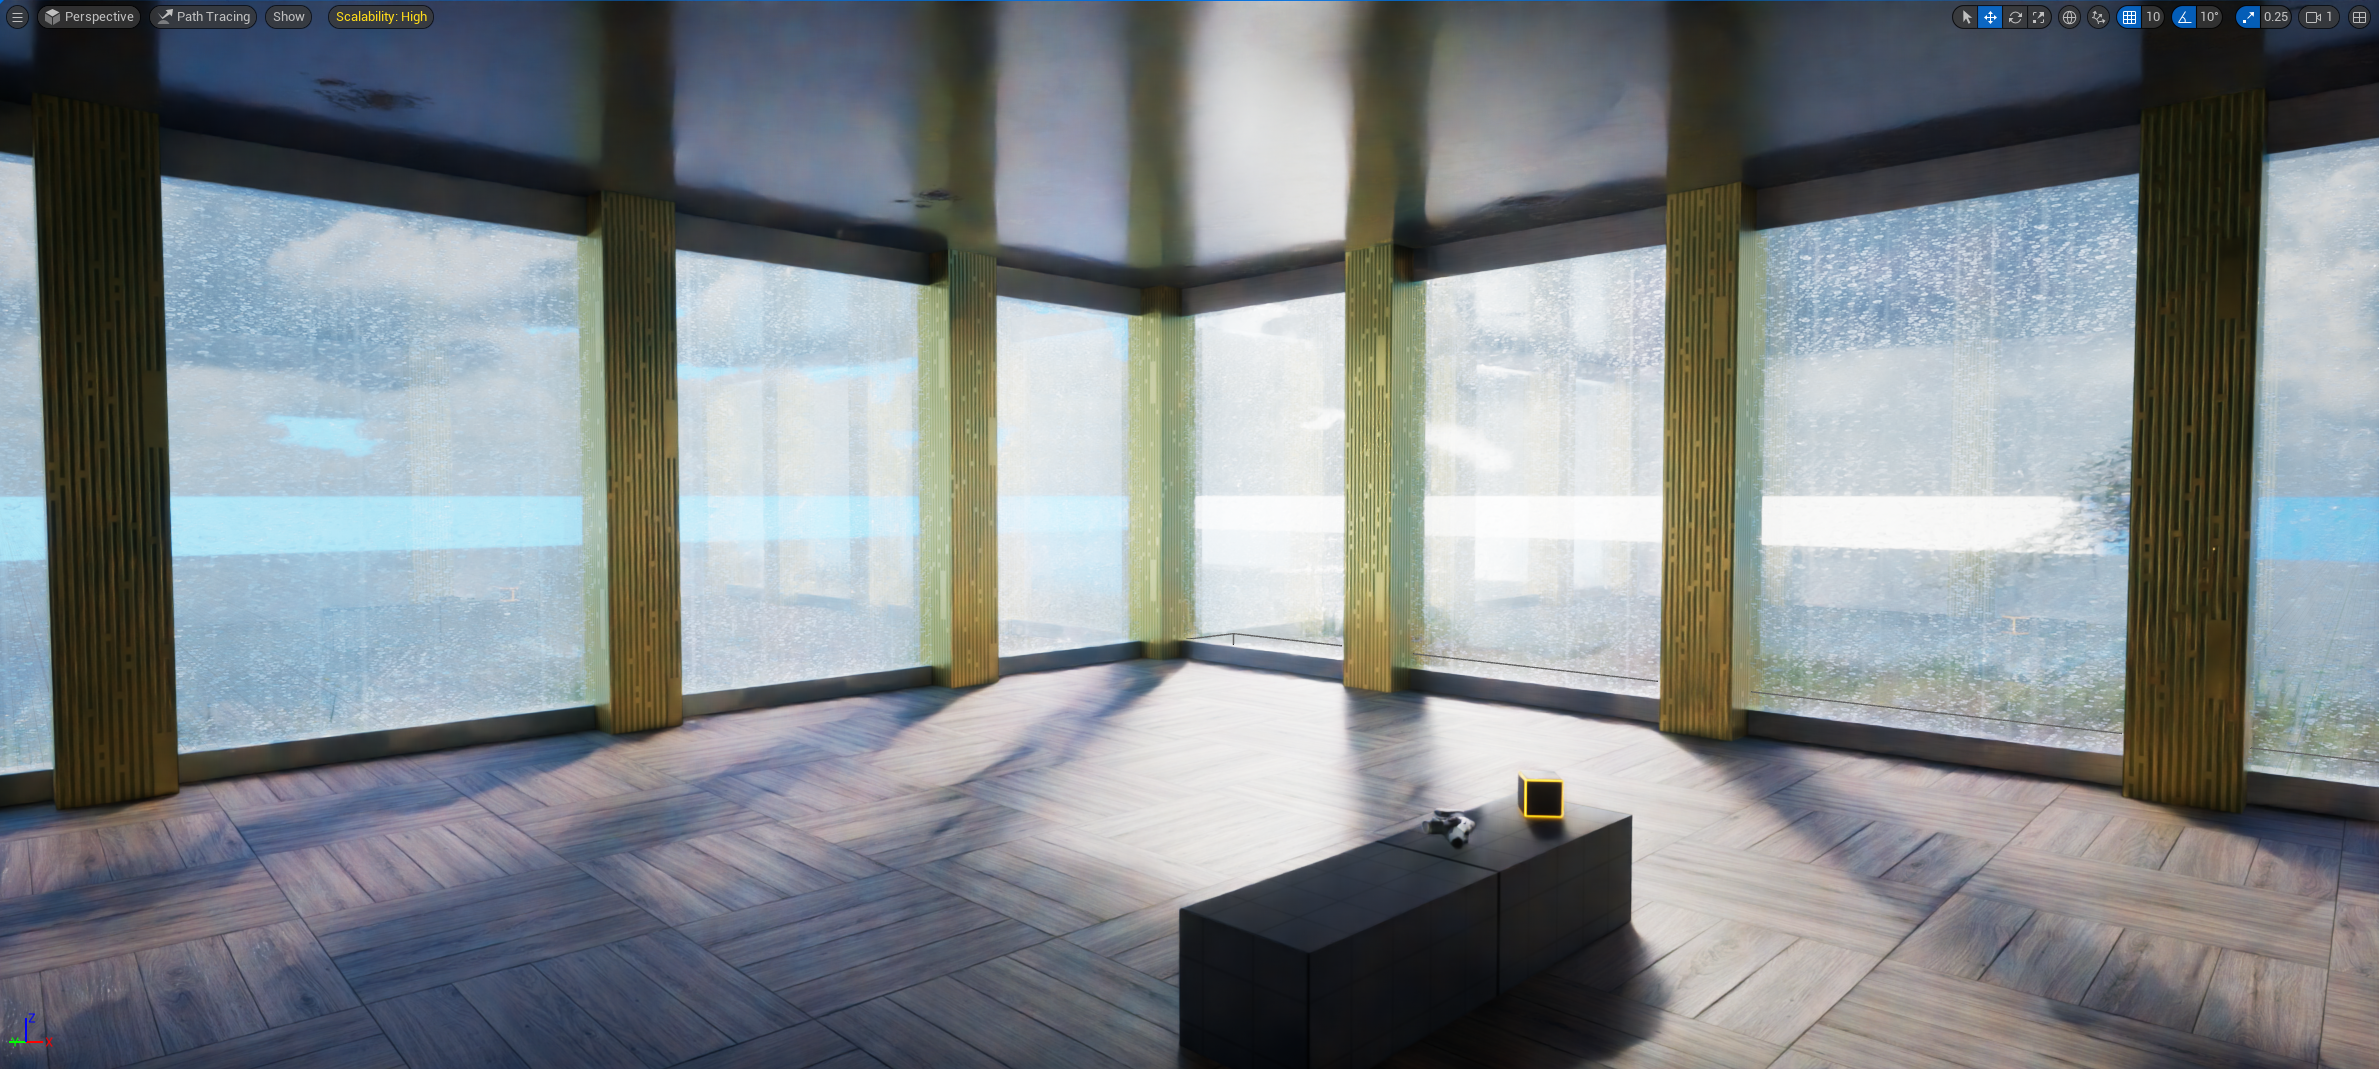
\includegraphics[width=\linewidth, height=6cm]{continut/capitol3/figuri/ray2.png}
        \label{fig:Ray Tracing}
    \end{subfigure}
    \hfill
    \begin{subfigure}{0.49\textwidth}
        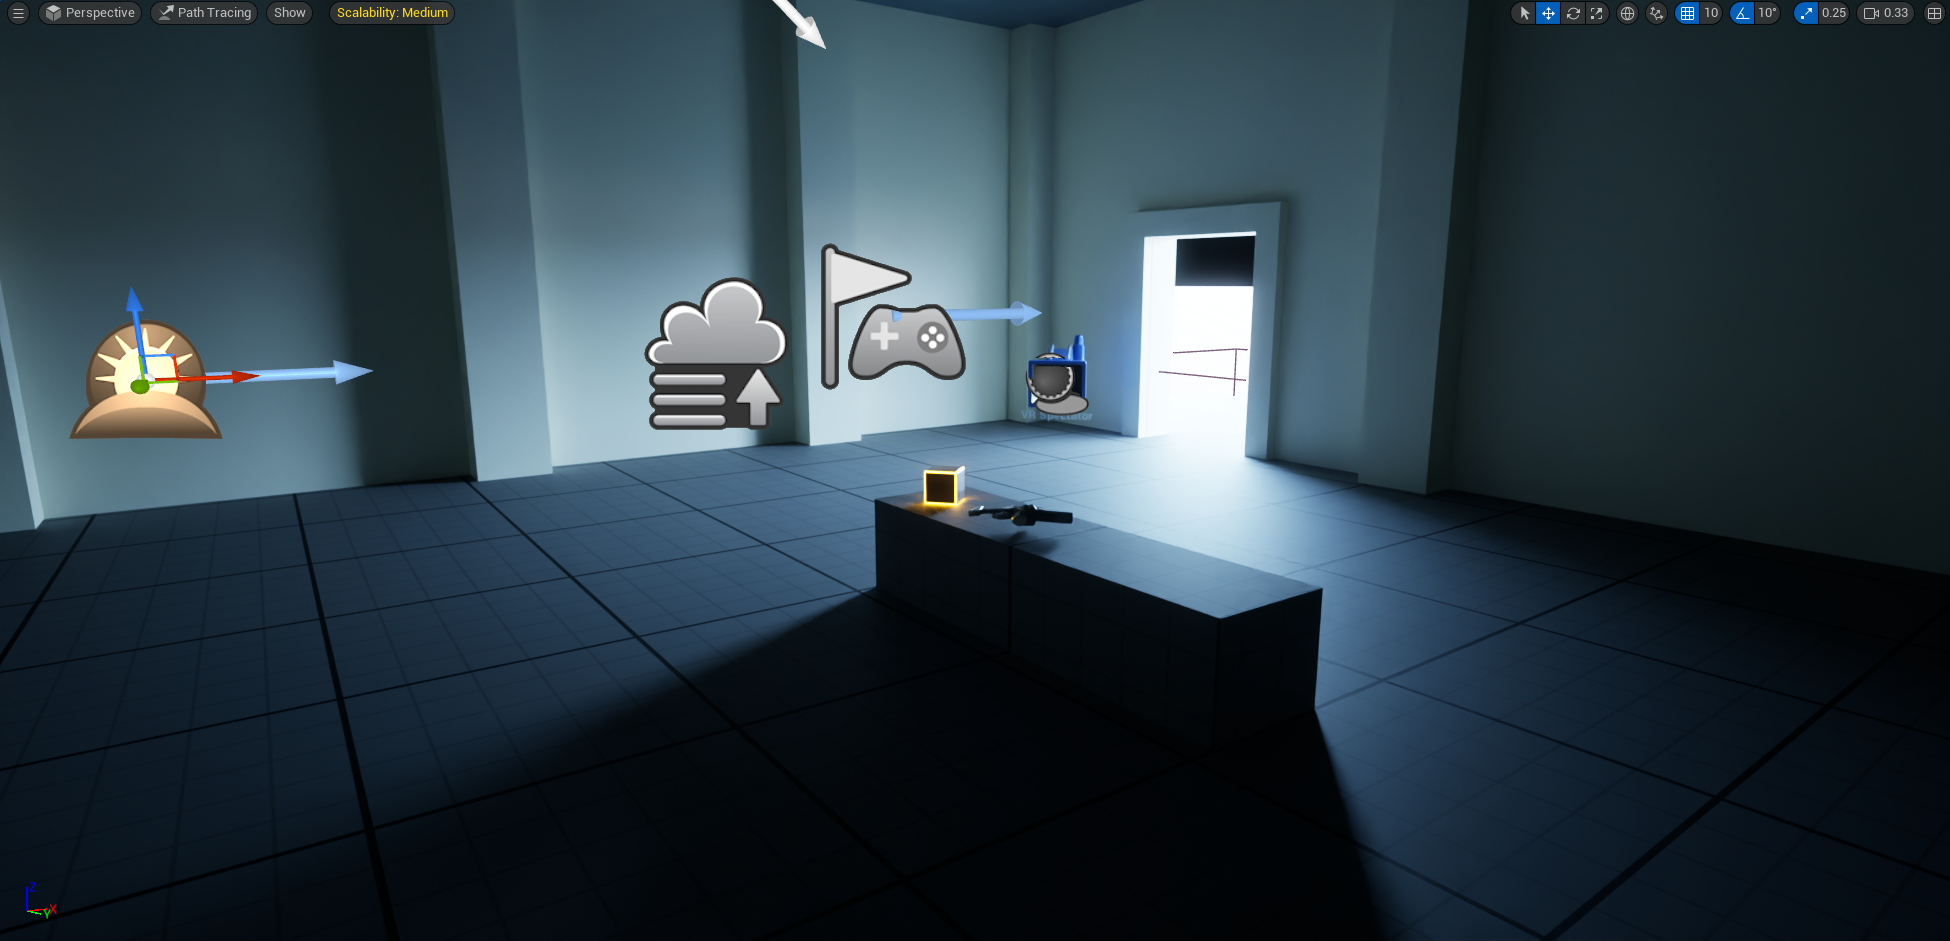
\includegraphics[width=\linewidth, height=6cm]{continut/capitol3/figuri/ray_traced.png}
        \label{fig:Ray Tracing}
    \end{subfigure}
    \caption{Lumina din interior și exterior - teste inițiale}
\end{figure}

În zona exterioară, iluminarea simulează condițiile din timpul amiezii, cu un ambient luminos constant. Soarele este poziționat într-un unghi static optim, astfel încât fiecare model 3D să poată fi observat cu ușurință, fără umbre prea dure sau zone excesiv de întunecate. Nu a fost implementat un ciclu de zi-noapte, deoarece durata medie estimată de explorare a experienței este de aproximativ 10 minute - un interval prea scurt pentru a justifica rotația dinamică a soarelui sau tranziții de iluminare. Astfel, soarele rămâne fix pe cer pe tot parcursul sesiunii.

La interior, arhitectura a fost inițial proiectată cu multe ferestre, însă s-a renunțat ulterior la această soluție în favoarea iluminării artificiale controlate. Ferestrele au fost acoperite parțial sau complet pentru a preveni interferența luminii naturale cu sursele de lumină plasate strategic în muzeu. Astfel, iluminarea interioară se bazează exclusiv pe corpuri de iluminat de tip neon (tuburi fluorescente), amplasate atât deasupra exponatelor, cât și pe tavan.

Această abordare are mai multe avantaje. În primul rând, asigură o distribuție uniformă a luminii, evitând zonele prea întunecate sau prea luminate. În al doilea rând, permite evidențierea efectelor de ray tracing în timp real – reflexii, umbre dinamice și iluminare globală indirectă - care contribuie major la realismul vizual. Fiecare sursă de lumină a fost calibrată pentru a evidenția obiectele din jurul ei, punând accent pe detalii, forme și materiale.

Anumite zone ale muzeului sunt intenționat mai intens luminate pentru a atrage atenția asupra unor expoziții cheie sau pentru a accentua dramatismul scenei. Această variație de intensitate luminează contextul narativ și oferă o experiență mai dinamică.

\begin{figure} [htp] 
\centering 
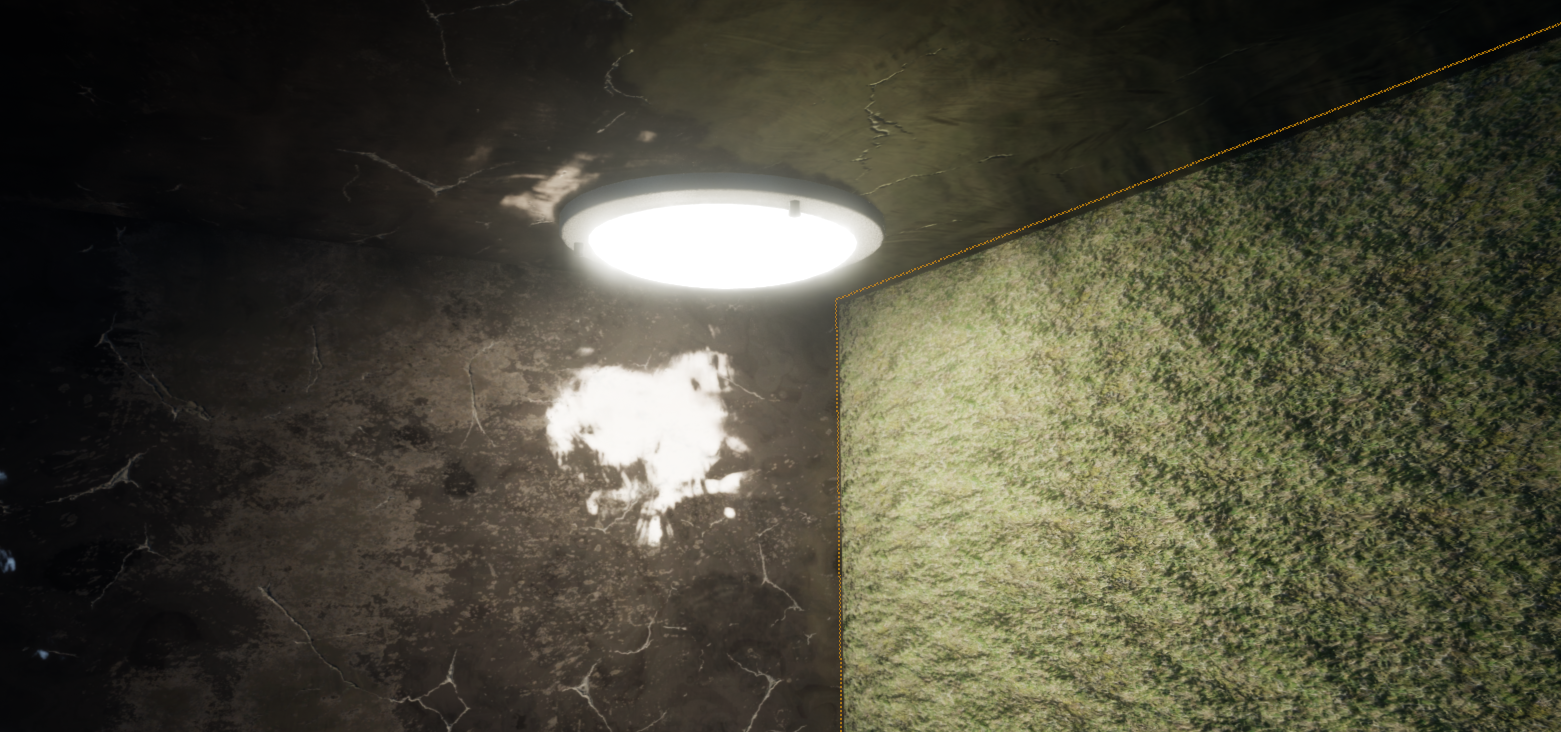
\includegraphics [width=12cm]
{continut/capitol3/figuri/rayBIMtraced.png} 
\label{fig:Ray Tracing} 
    \caption{Ray Tracing}
\end{figure}

Totuși, în unele cazuri pot apărea mici artefacte vizuale, precum flickering-ul luminii (palpitații sau variații neașteptate de intensitate), cauzate de interacțiuni între geometriile scenei și modul în care lumina este calculată în timp real. Astfel de probleme apar rareori și nu afectează semnificativ experiența generală, mai ales că majoritatea situațiilor au fost optimizate în faza de testare.

De menționat că sistemul de iluminare a fost gândit pentru a fi compatibil cu standardele performanței în VR. Deși iluminarea în timp real oferă rezultate vizuale excelente, aceasta poate fi costisitoare din punct de vedere al resurselor, motiv pentru care s-au realizat compromisuri controlate: s-a preferat folosirea static și stationary lights acolo unde a fost posibil, și s-a limitat numărul de surse dinamice per cameră pentru a menține fluiditatea aplicației.

Iluminarea în VR Museum nu are doar un rol funcțional, ci și estetic și educațional, contribuind activ la conturarea atmosferei generale și la accentuarea punctelor de interes din cadrul turului virtual.

\section{Expoziții}

\begin{figure}[h!]
    \centering
    \begin{subfigure}{0.49\textwidth}
        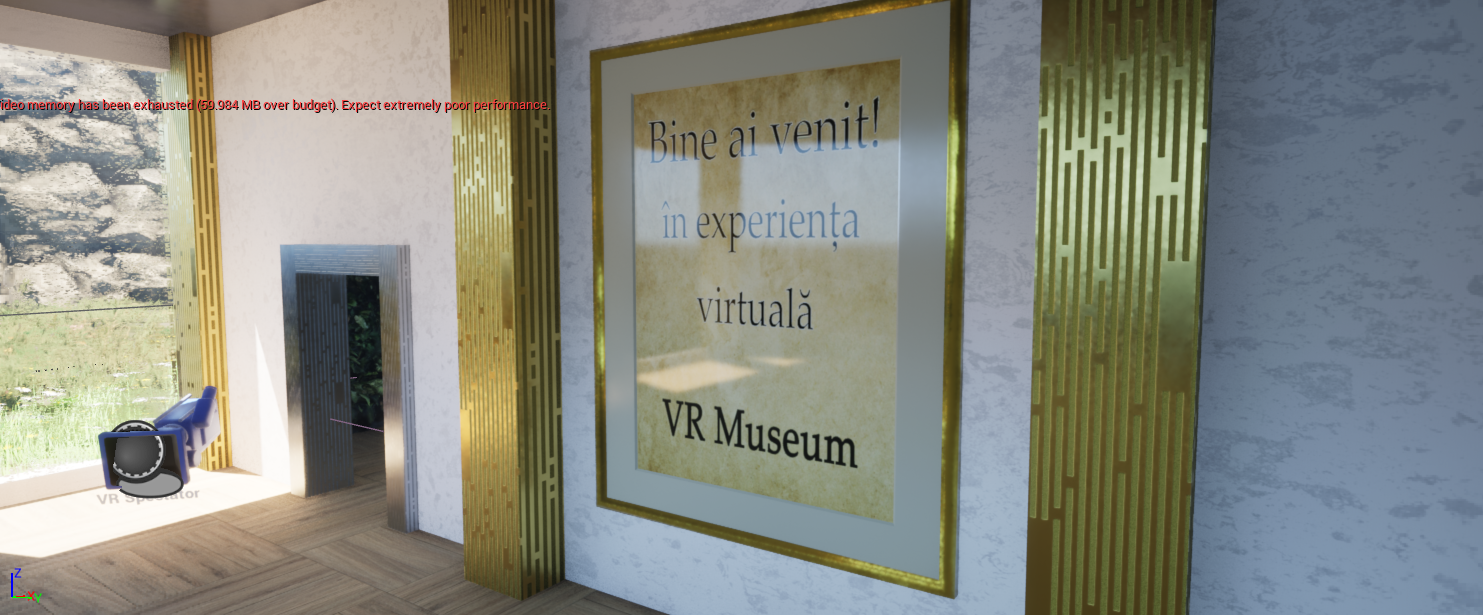
\includegraphics[width=\linewidth, height=6cm]{continut/capitol3/figuri/panel.png}
        \label{fig:Terrain mapping}
    \end{subfigure}
    \hfill
    \begin{subfigure}{0.49\textwidth}
        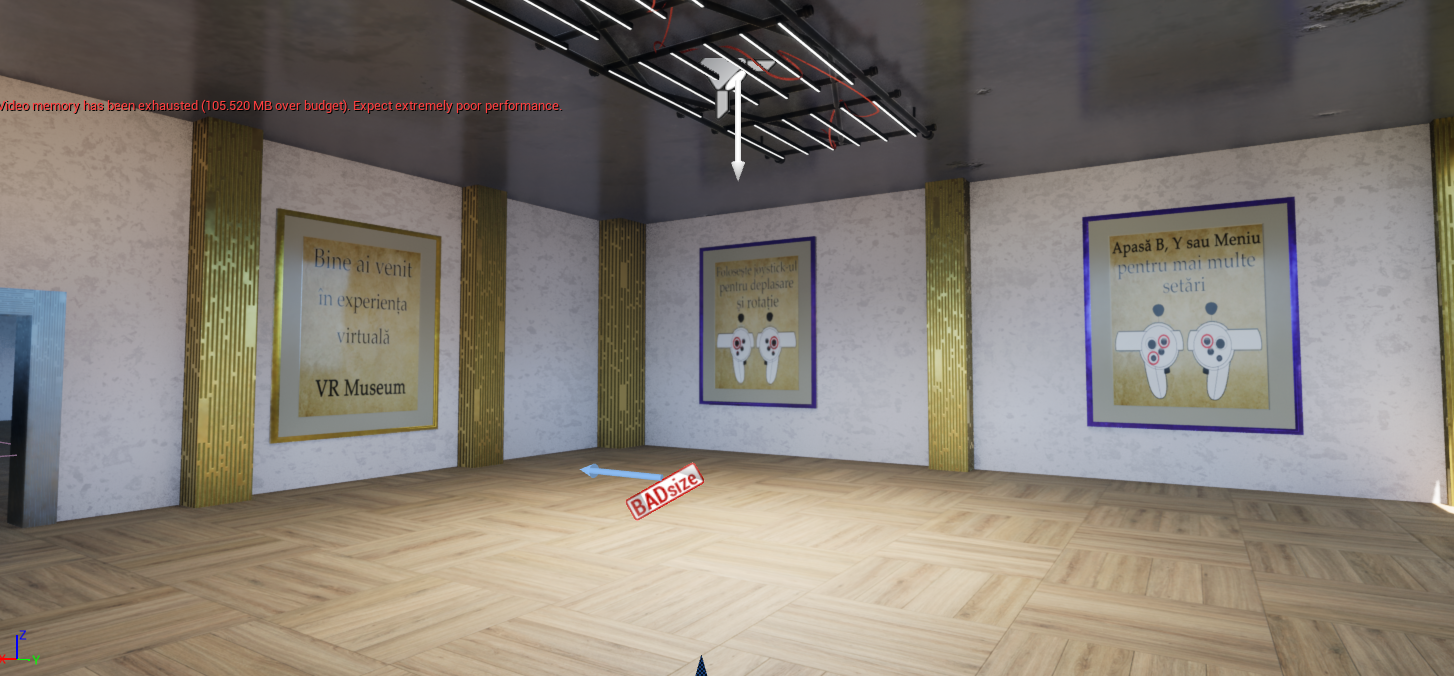
\includegraphics[width=\linewidth, height=6cm]{continut/capitol3/figuri/panel2.png}
        \label{fig:Terrain mapping}
    \end{subfigure}
    \caption{Camera de start}
\end{figure}

În cadrul muzeului virtual sunt integrate mai multe expoziții tematice, fiecare amplasată în încăperi distincte, cu o identitate vizuală și informațională proprie. Distribuția acestora este gândită astfel încât utilizatorul să parcurgă un traseu progresiv, în care imersiunea și gradul de interacțiune cresc odată cu avansarea prin spațiul muzeal.

Camera de inițializare (start room) are rolul de a familiariza utilizatorul cu sistemul de control, printr-o zonă special dedicată testării mișcării, orientării spațiale și interacțiunilor de bază. Aici pot fi observate instrucțiuni vizuale, meniu simplificat și elemente interactive de antrenament, toate într-un mediu neutru, menit să introducă vizitatorul în experiență fără disconfort.

\begin{figure}[h!]
    \centering
    \begin{subfigure}{0.49\textwidth}
        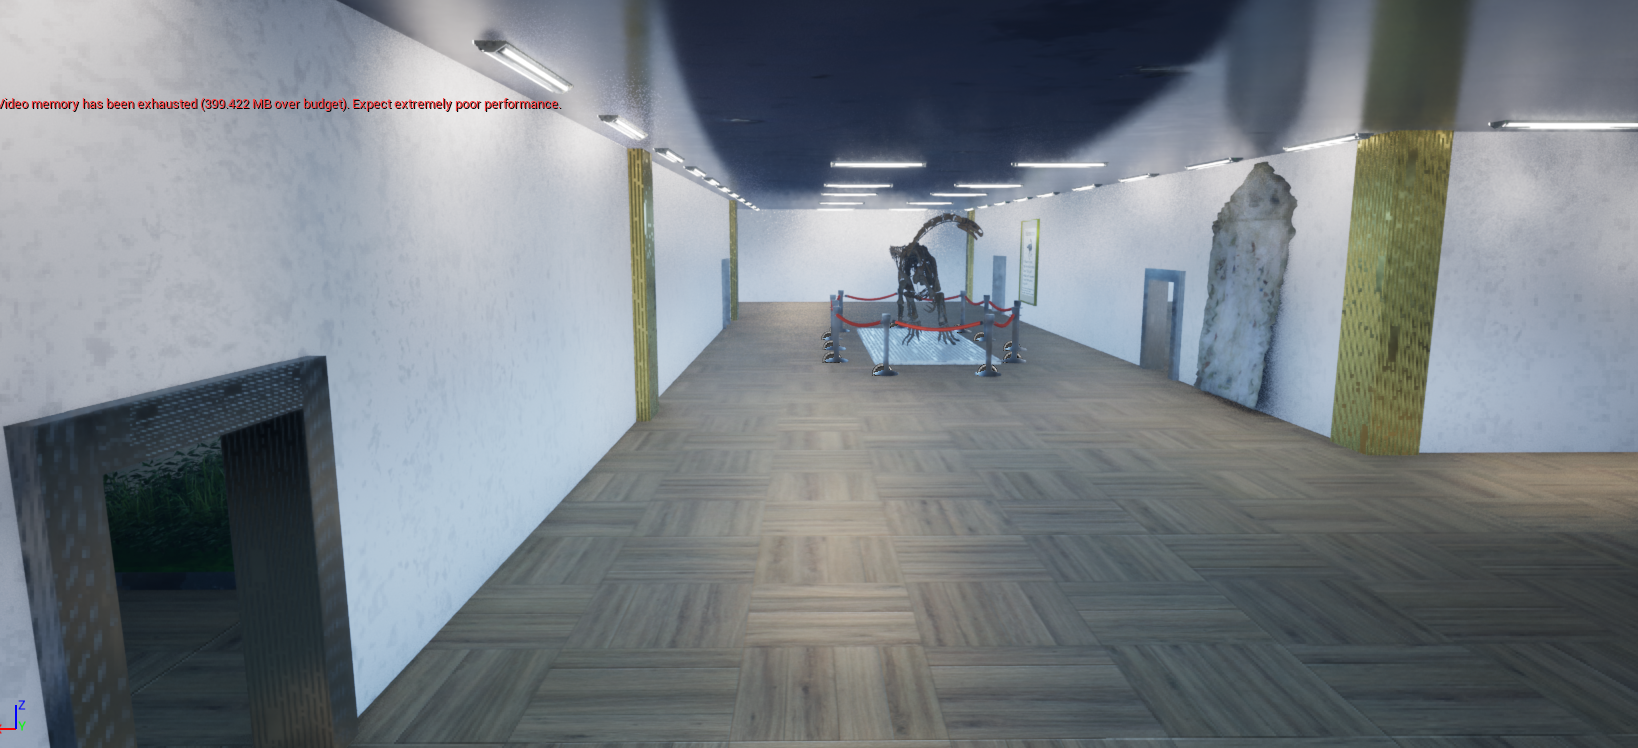
\includegraphics[width=\linewidth, height=6cm]{continut/capitol3/figuri/hol.png}
        \label{fig:Terrain mapping}
    \end{subfigure}
    \hfill
    \begin{subfigure}{0.49\textwidth}
        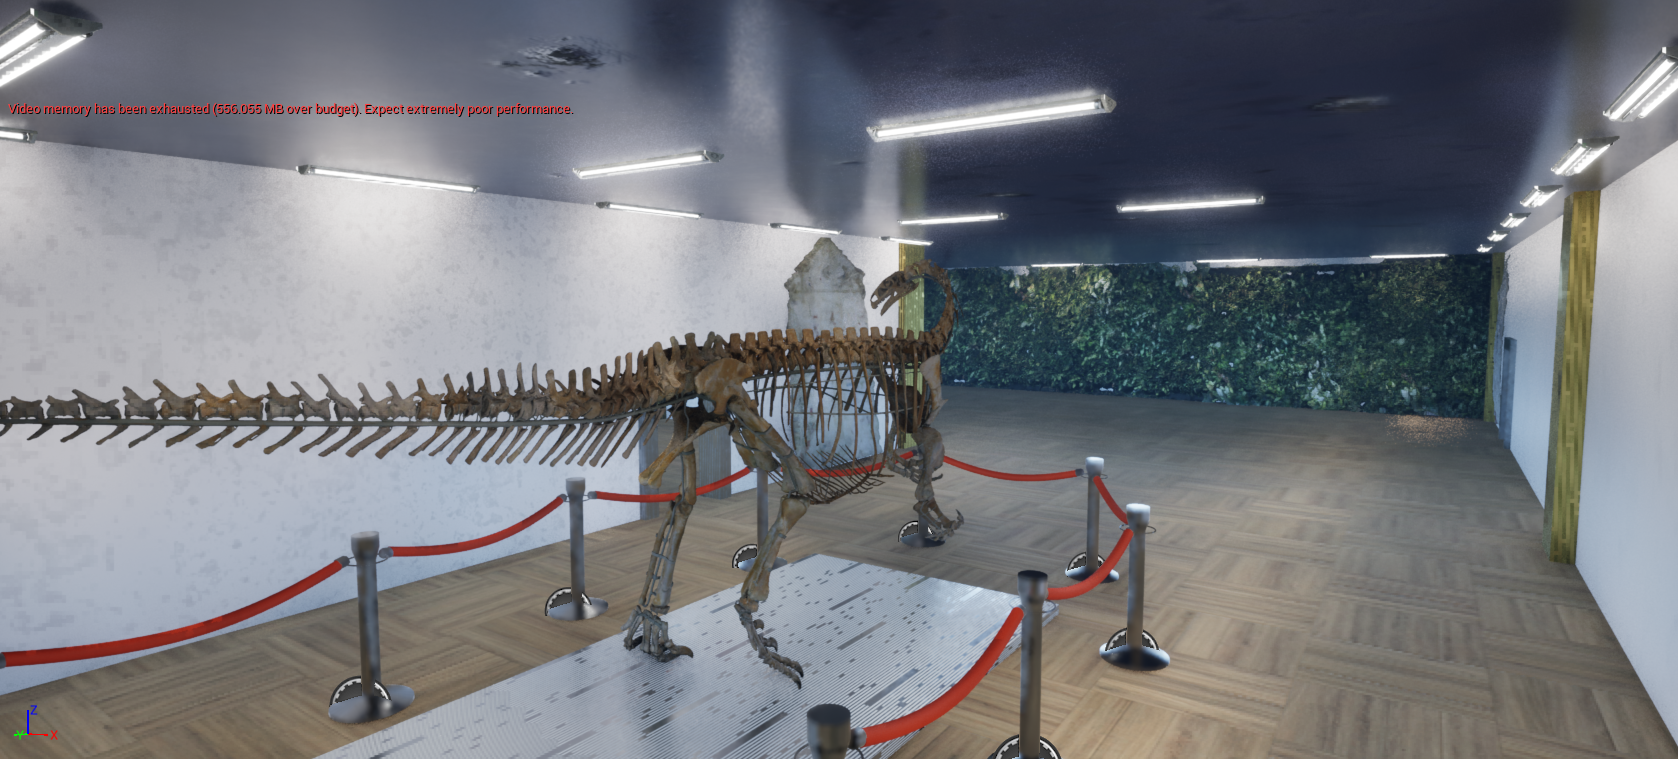
\includegraphics[width=\linewidth, height=6cm]{continut/capitol3/figuri/hol2.png}
        \label{fig:Terrain mapping}
    \end{subfigure}
    \caption{Holul muzeului}
\end{figure}

Urmează holul central, un spațiu amplu decorat cu vegetație 3D, lumină volumetrică și efecte ambientale dinamice. Holul servește drept nod de legătură către celelalte săli și adăpostește o piesă centrală remarcabilă: un schelet de Paleosaurus, modelat cu detalii fine și iluminat cu surse direcționale pentru evidențierea structurii osoase.

\begin{figure}[h!]
    \centering
    \begin{subfigure}{0.49\textwidth}
        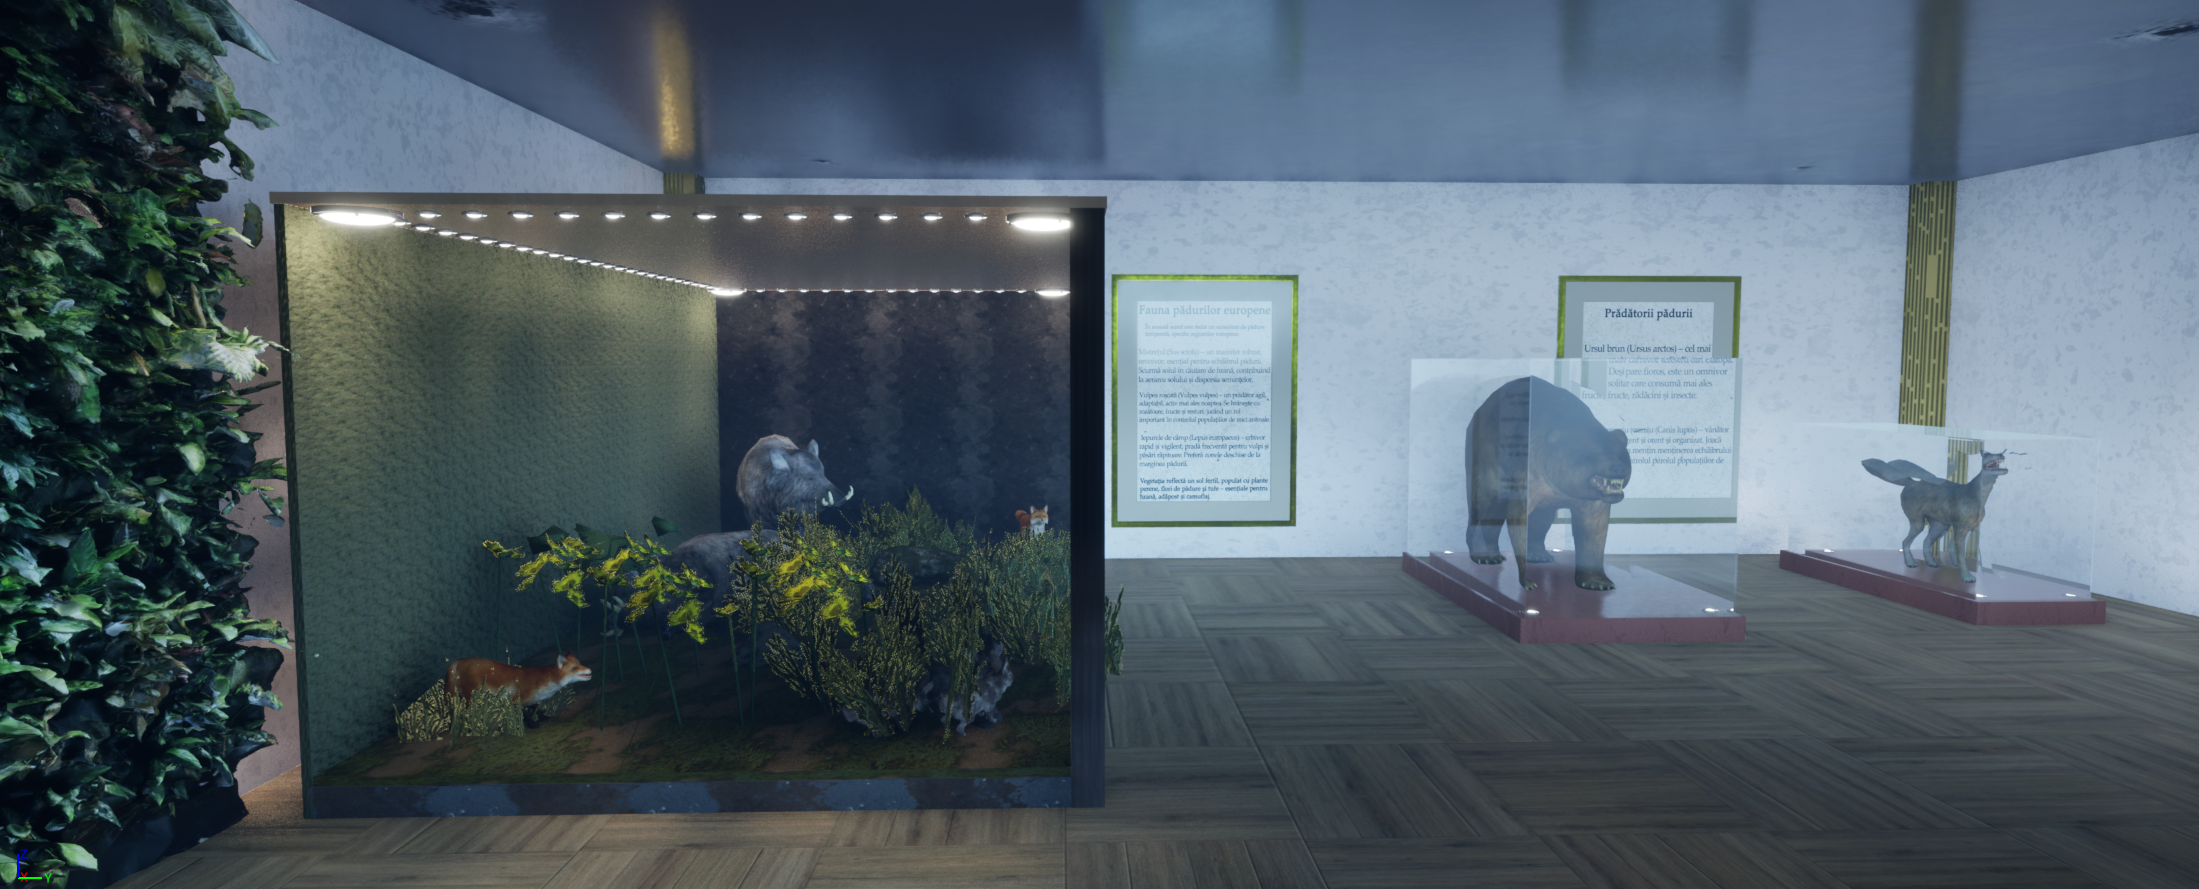
\includegraphics[width=\linewidth, height=6cm]{continut/capitol3/figuri/camera1.png}
        \label{fig:Room1}
    \end{subfigure}
    \hfill
    \begin{subfigure}{0.49\textwidth}
        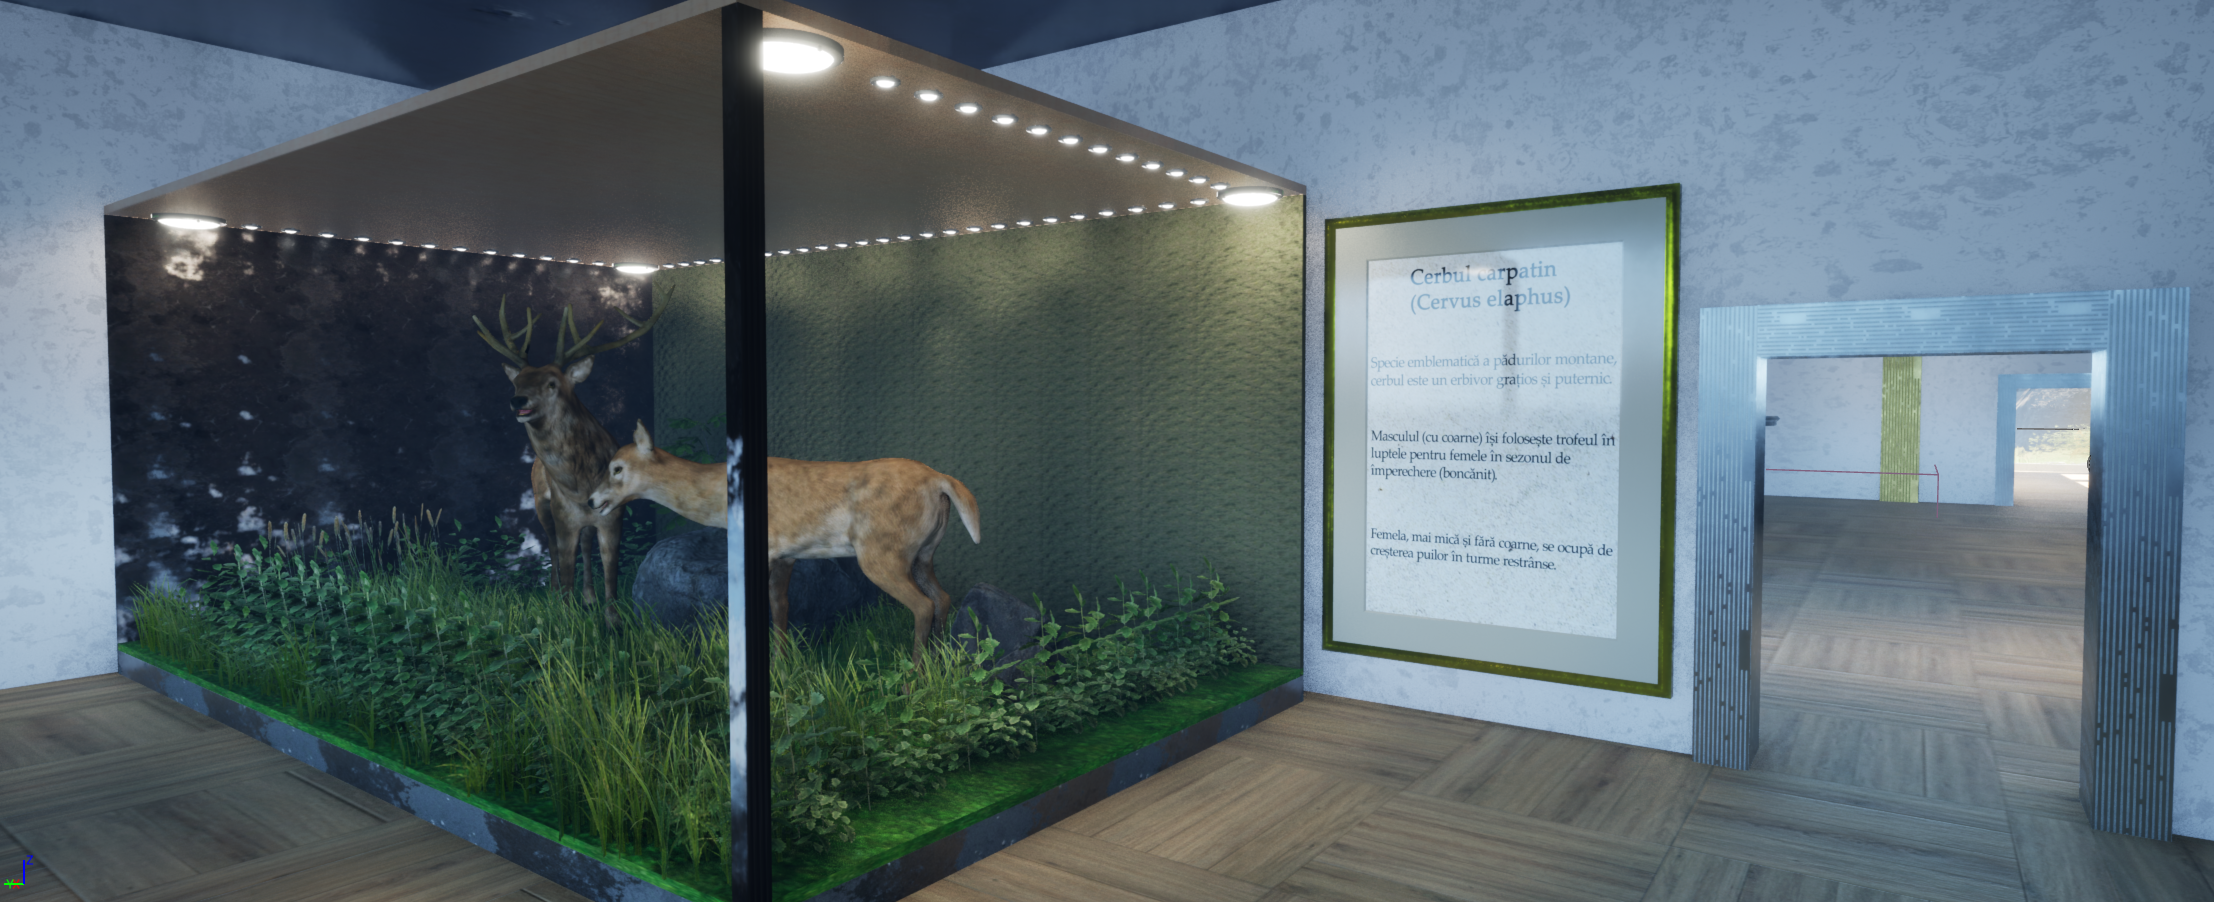
\includegraphics[width=\linewidth, height=6cm]{continut/capitol3/figuri/camera1_2.png}
        \label{fig:Room1}
    \end{subfigure}
    \caption{Camera 1}
\end{figure}

Prima cameră de expoziție este dedicată mamiferelor terestre. Aceasta conține modele 3D realiste ale unor specii sălbatice, atât prădători cât și ierbivore, amplasate în poziții naturale. Fiecare exemplar este însoțit de un panou informativ digital, ce conține date despre habitat, comportament și rolul său în lanțul trofic. Panourile sunt concepute astfel încât informațiile să fie declanșate la apropierea utilizatorului.

\begin{figure}[h!]
    \centering
    \begin{subfigure}{0.49\textwidth}
        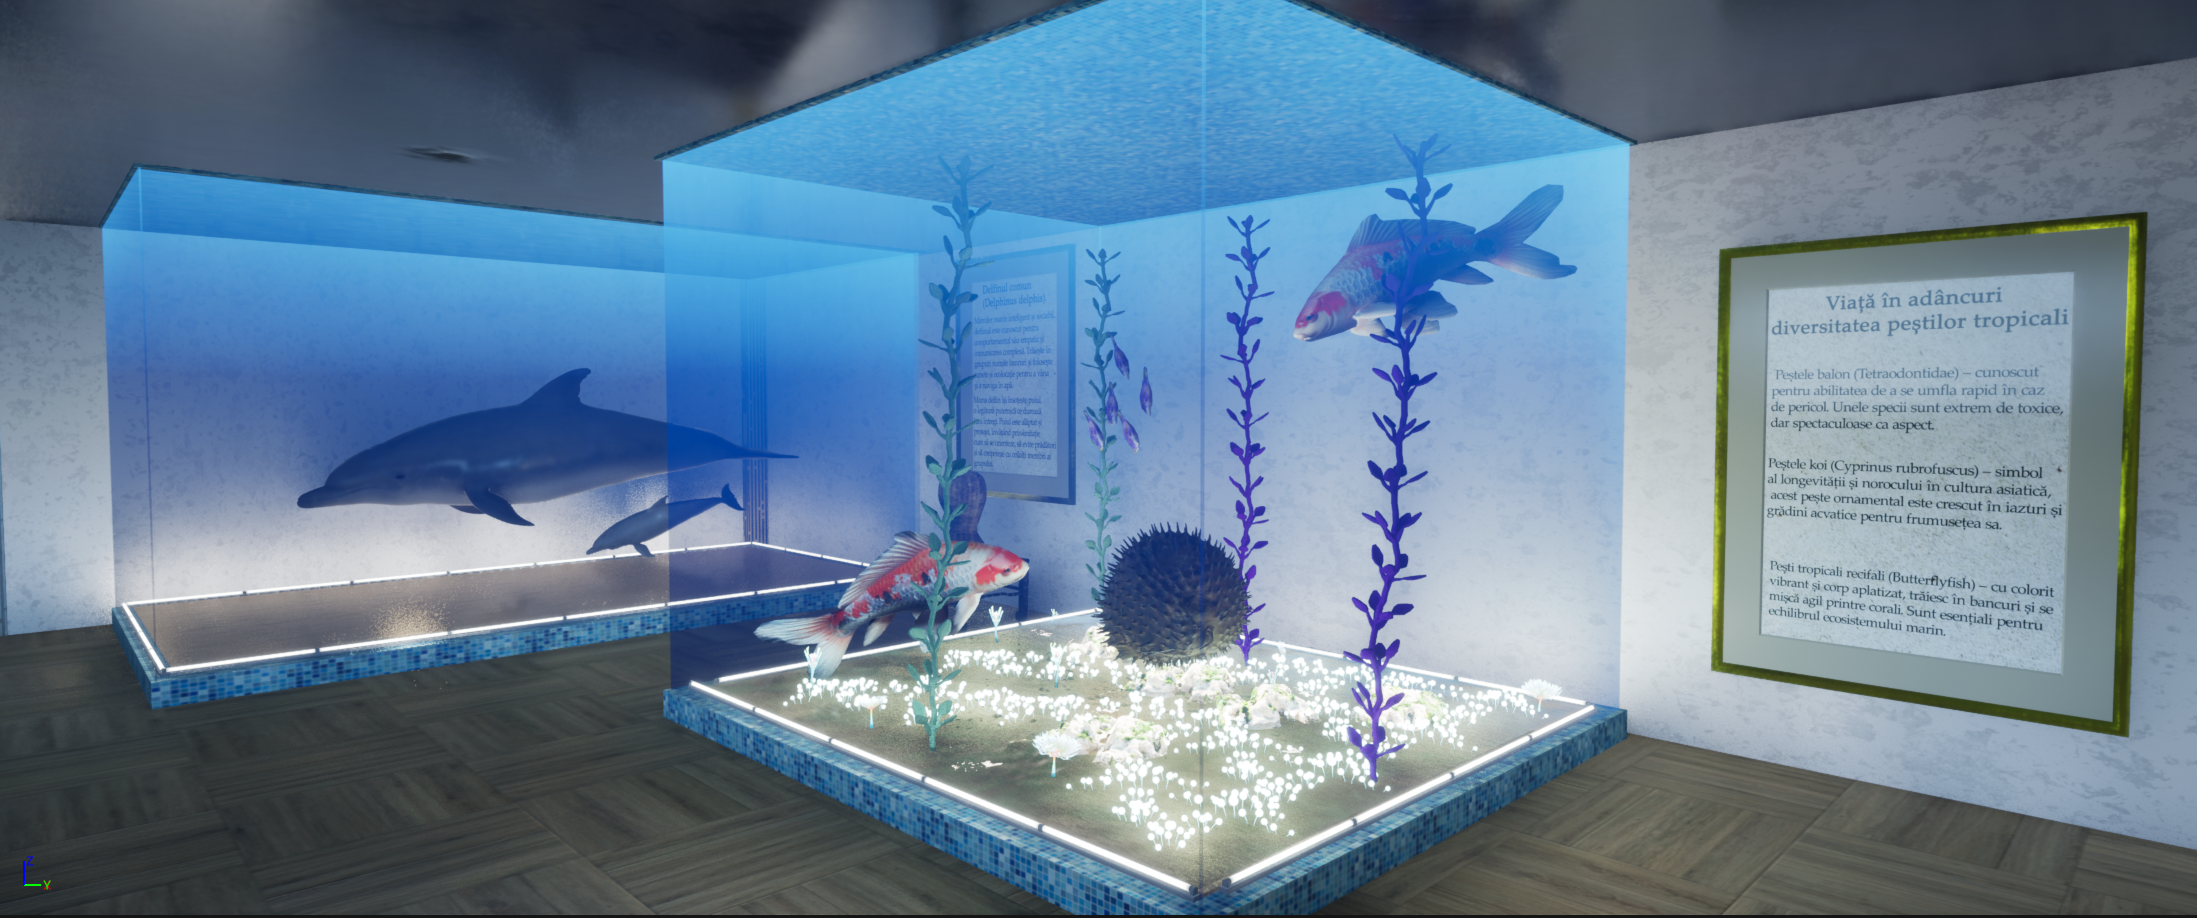
\includegraphics[width=\linewidth, height=6cm]{continut/capitol3/figuri/camera_2.png}
        \label{fig:Room2}
    \end{subfigure}
    \hfill
    \begin{subfigure}{0.49\textwidth}
        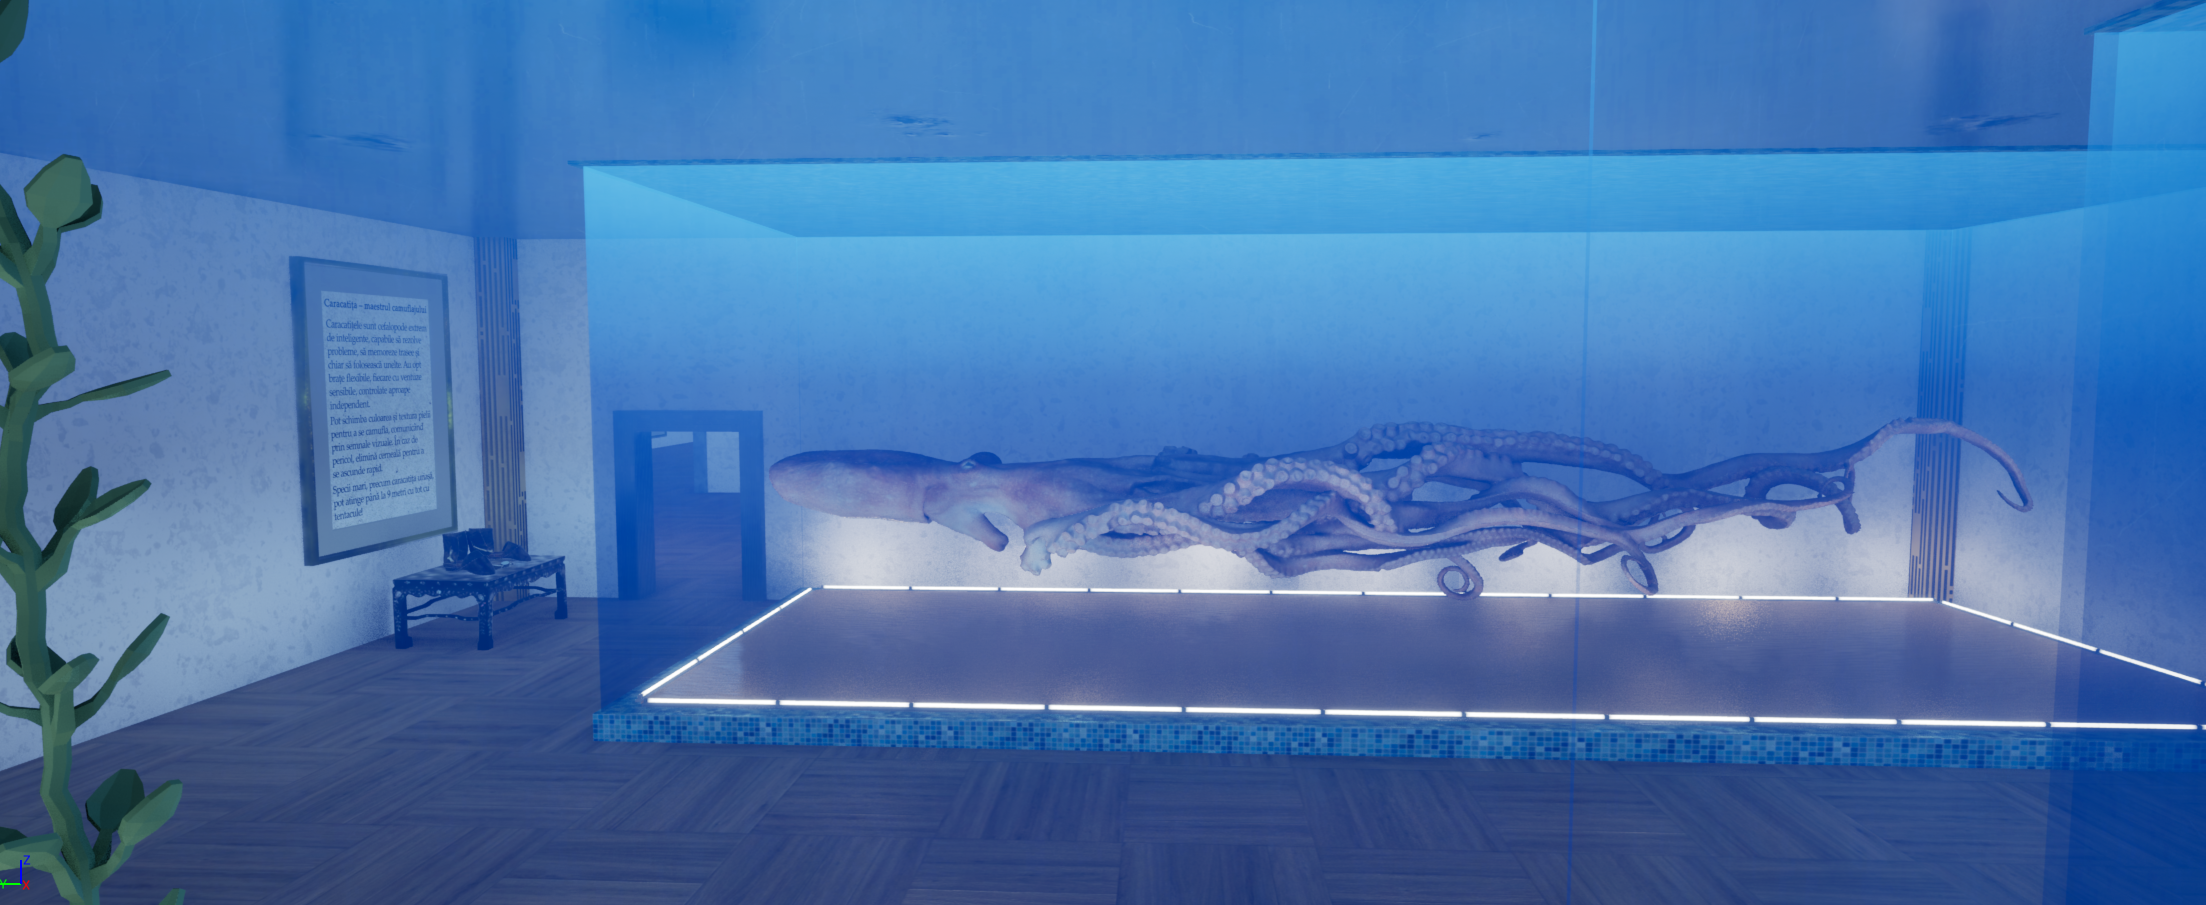
\includegraphics[width=\linewidth, height=6cm]{continut/capitol3/figuri/camera2_2.png}
        \label{fig:Room2}
    \end{subfigure}
    \caption{Camera 2}
\end{figure}

În continuare, camera acvatică oferă o tranziție către mediile subacvatice. Aici pot fi întâlnite un grup familial de delfini (mamă și pui), o caracatiță de dimensiuni mari și un acvariu digital interactiv cu pești tropicali. Pe lângă fauna marină, expoziția include și o serie de obiecte tradiționale folosite în pescuit, precum capcane din lemn, plase vechi și cârlige artizanale, toate recreate digital pe baza surselor istorice.

\newpage 
În partea opusă se află o încăpere mai spațioasă, destinată unei colecții de obiecte istorice de utilitate practică: unelte, recipiente, instrumente de vânătoare și chiar obiecte de divertisment arhaice. Acestea nu sunt prezentate la scară reală, ci au fost redimensionate pentru o mai bună lizibilitate și încadrare vizuală în spațiul VR. Obiectele sunt grupate tematic, fiecare fiind însoțit de o scurtă descriere contextuală – unele cu fundal audio explicativ.

\begin{figure} [htp] 
\centering 
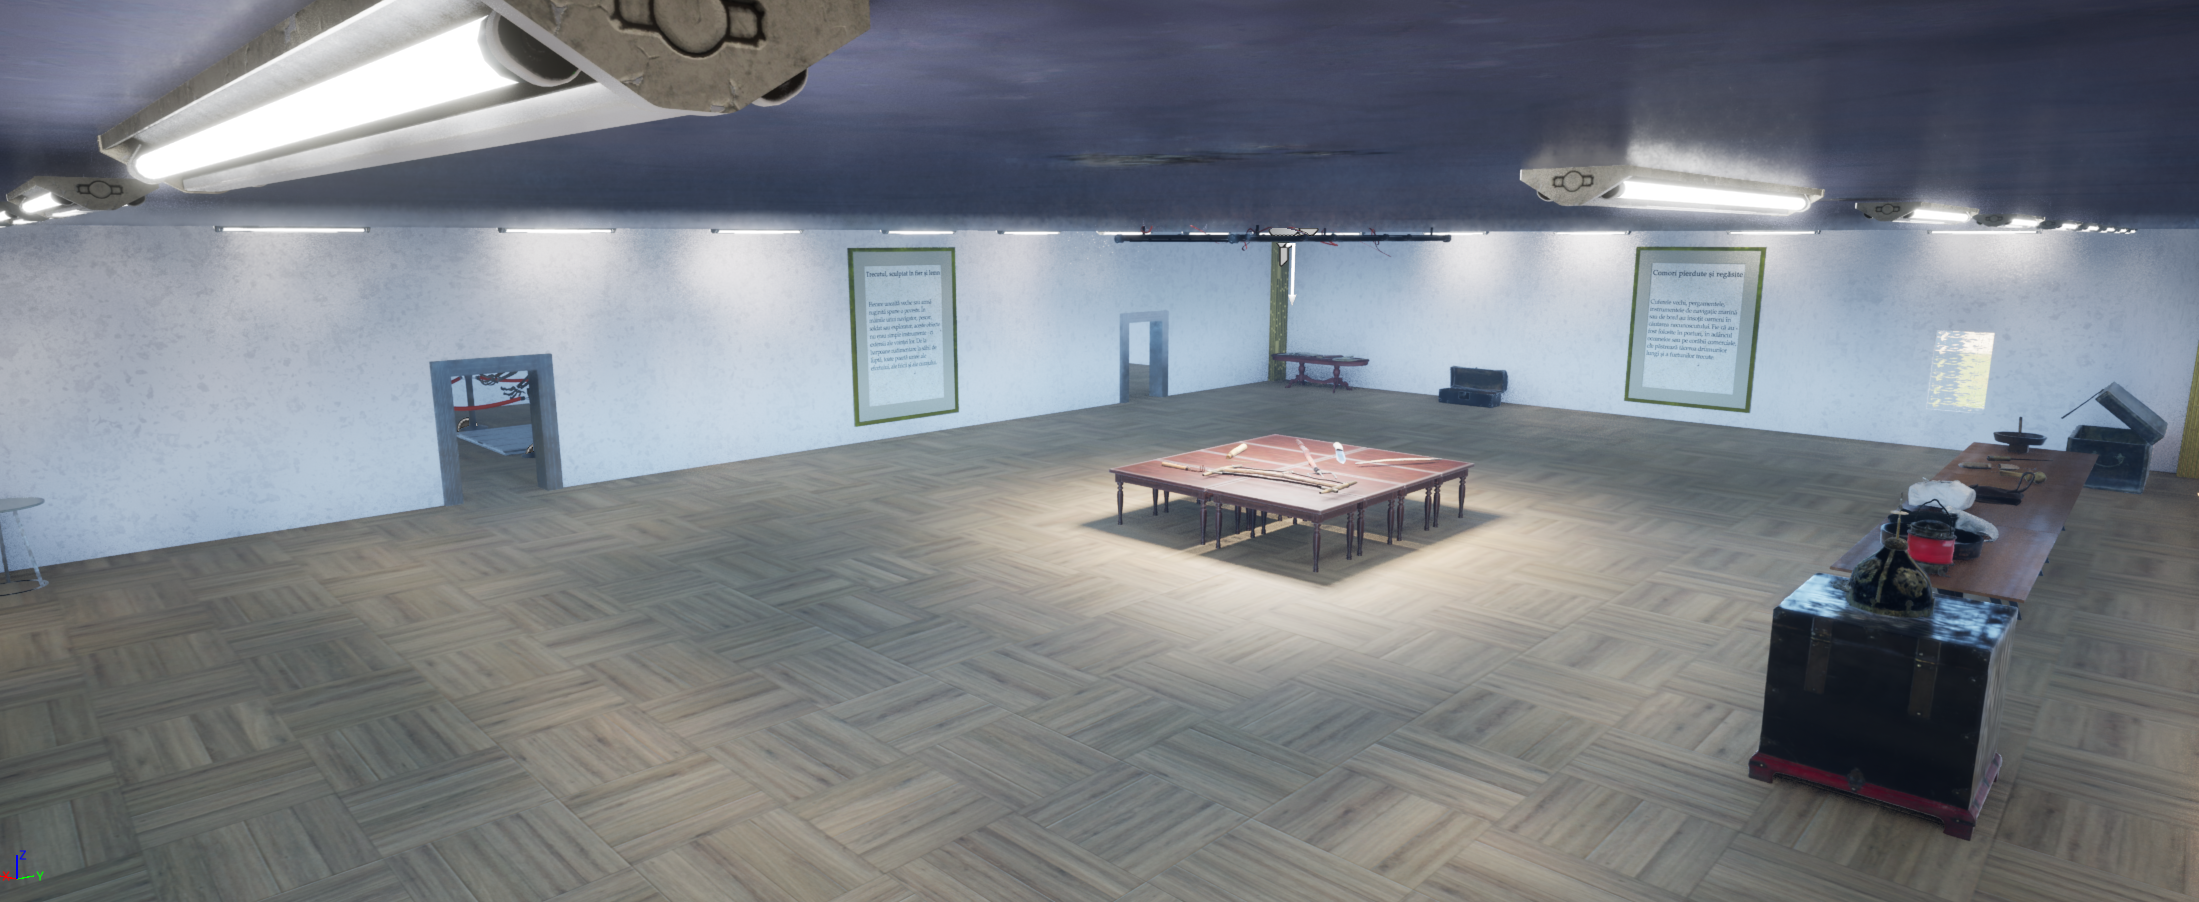
\includegraphics [width=12cm]
{continut/capitol3/figuri/iteme.png} 
\label{fig:Room3} 
    \caption{Camera 3}
\end{figure}

\section{VR Pawn}

\section{Movement}

\section{Meniul principal și cel de setări}

\section{Cerințele utilizatorului final}

Utilizatorii finali ai aplicației VR Museum sunt persoane interesate de cunoaștere, curioase să exploreze un spațiu cultural într-un mod modern și accesibil. Fie că vorbim despre elevi, studenți, cadre didactice sau persoane pasionate de știință, așteptările acestora se axează pe trei direcții majore: ușurința în utilizare, valoarea educațională a conținutului și imersiunea oferită de experiența VR.

Din punct de vedere al folosirii, VR Museum are un grad scăzut de complexitate, datorită instrucțiunilor incluse în experiența virtuală. Setările pot fi accesate cu ușurință prin apăsarea butoanelor de pe controlerele VR, fie pe cel din mâna dreaptă, fie pe cel din stânga, iar navigarea se realizează simplu și intuitiv cu ajutorul joystick-ului.

Atmosfera trăită în VR Museum este una plăcută și memorabilă; muzeul virtual reușește să redea senzația unui spațiu fizic real, cu o iluminare dinamică adaptată cadrului, sunete ambientale discrete și plăcute, precum și un nivel de detaliu grafic ridicat care contribuie semnificativ la senzația de imersiune.

Aplicația rulează fluent pe majoritatea sistemelor compatibile cu VR. Desigur, nivelul detaliilor vizuale poate varia în funcție de specificațiile tehnice ale echipamentului folosit, însă experiența generală rămâne constantă și de calitate, indiferent de configurație.

Utilizatorii s-ar putea aștepta ca o astfel de aplicație să fie disponibilă contra cost, având în vedere efortul de dezvoltare și numărul mare de ore de muncă investite. Cu toate acestea, VR Museum este oferită gratuit, în format open-source, pentru a putea fi utilizată și extinsă liber în scopuri educaționale, demonstrative sau culturale. Codul sursă este accesibil, permițând dezvoltatorilor să adauge noi funcționalități, să îmbunătățească interfața sau să creeze versiuni personalizate ale muzeului în funcție de propriile nevoi.